\documentclass[10pt]{article}
\usepackage[accepted]{tmlr}
\usepackage[utf8]{inputenc}
\usepackage[T1]{fontenc}
\usepackage{lmodern}
\usepackage{xcolor}
\definecolor{purple}{RGB}{128,0,128}
\definecolor{gray}{gray}{0.45}


\usepackage{amsmath,amssymb,amsthm,mathtools}
\numberwithin{equation}{section}


\usepackage{microtype}
\usepackage{graphicx}

\usepackage{subcaption}
\usepackage{booktabs}
\usepackage{placeins}

\graphicspath{{figs/}{figs/cifar10/}{plots/}{results-stressed-cap80/plots/}{paper-extra-experiments/plots/}{relevance-demo/plots/}}


\usepackage{enumitem}
\usepackage{listings}

\usepackage{tabularx}
\usepackage{ragged2e}
\usepackage{xspace}


\lstset{
language=Python,
basicstyle=\ttfamily\footnotesize,
breaklines=true,
breakatwhitespace=false,
showstringspaces=false,
captionpos=b,
frame=single,
numbers=left,
numberstyle=\tiny\color{gray},
keywordstyle=\color{blue},
commentstyle=\color{green!60!black},
stringstyle=\color{purple}
}

\usepackage{hyperref}
\hypersetup{
colorlinks=true,
linkcolor=blue!70!black,
citecolor=blue!70!black,
urlcolor=blue!70!black,
pdftitle={Finite-Step Sinkhorn Certificates for Nonnegative Stream-Mixing Products},
pdfauthor={Maksim Kosmakov}
}


% --- THEOREMS ---
\theoremstyle{plain}
\newtheorem{theorem}{Theorem}[section]
\newtheorem{proposition}[theorem]{Proposition}
\newtheorem{corollary}[theorem]{Corollary}
\newtheorem{lemma}[theorem]{Lemma}
\newtheorem{assumption}[theorem]{Assumption}
\newtheorem{fact}[theorem]{Fact}
\newtheorem{claim}[theorem]{Claim}

\theoremstyle{definition}
\newtheorem{definition}[theorem]{Definition}

\theoremstyle{remark}


% --- MACROS ---
\newcommand{\R}{\mathbb{R}}
\newcommand{\e}{\mathrm{e}}
\newcommand{\ones}{\mathbf{1}}
\newcommand{\cB}{\mathcal{B}}
\newcommand{\cP}{\mathcal{P}}
\newcommand{\diag}{\operatorname{diag}}
\newcommand{\tr}{\operatorname{Tr}}
\newcommand{\ip}[2]{\left\langle #1, #2 \right\rangle}
\newcommand{\norm}[1]{\left\lVert #1 \right\rVert}
\newcommand{\abs}[1]{\left\lvert #1 \right\rvert}
\newcommand{\Hres}{H_{\mathrm{res}}}
\newcommand{\Hpre}{H_{\mathrm{pre}}}
\newcommand{\Hpost}{H_{\mathrm{post}}}
\newcommand{\KL}{\operatorname{KL}}
\newcommand{\Ent}{\operatorname{Ent}}
\newcommand{\vecop}{\operatorname{vec}}
\newcommand{\Amax}{\texorpdfstring{\ensuremath{A_{\max}}}{Amax}\xspace}
\newcommand{\kobs}{\kappa_{\mathrm{obs}}}
\newcommand{\epstol}{\varepsilon_{\mathrm{tol}}}
\newcommand{\epsfloor}{\varepsilon_{\mathrm{floor}}}
\newcommand{\tstop}{t_{\mathrm{stop}}}
\newcommand{\tmax}{t_{\max}}

\title{Finite-Step Sinkhorn Certificates for Nonnegative Stream-Mixing Products}


\author{\name Maksim Kosmakov \email maksim.kosmakov@utoledo.edu \\
\addr The University of Toledo}

\def\month{11}
\def\year{2026}
\def\openreview{\url{https://openreview.net/forum?id=NyEeOl6Gn7}}

\date{}

\begin{document}
\raggedbottom
\maketitle
\begingroup
\renewcommand{\thefootnote}{}
\footnotetext{The author used OpenAI Codex for assistance with code development and debugging.
The author takes responsibility for all content.}
\endgroup

\begin{abstract}
We develop deterministic finite-step bounds for products of nonnegative
stream-mixing matrices in expanded-stream residual architectures, with
Manifold-Constrained Hyper-Connections as the motivating example. We study the
depth-wise mixer product
\[
        T_L=\Hres^{(L)}\Hres^{(L-1)}\cdots \Hres^{(1)}
\]
and bound its forward and backward induced-norm gains. For entrywise
nonnegative mixers, row and column marginal defects directly control the
corresponding induced norms. These certificates concern the mixer pathway;
full-network stability additionally depends on the nonlinear residual branches.
In the column-then-row Sinkhorn order, exact row
sums give layerwise forward control, while the output column defect gives
\[
 \|T_L\|_1\le
 \min\Bigl\{\prod_{\ell=1}^L(1+\varepsilon_c^{(\ell)}),\,n\Bigr\},
\]
where \(n\) is a structural ceiling. We complement this product bound with a
telescoping refinement and a depth-uniform Dobrushin certificate under uniform
scrambling. A Hilbert-projective argument converts logit dynamic range,
temperature, and a finite Sinkhorn step cap into a conservative backward
mixer-path budget, while matrix-specific local analysis gives the asymptotic
rate \(\sigma_2(P)^2\). Numerical diagnostics examine marginal defects,
realized and certified gains, finite-step calibration, cap failures, and
normalization cost in matched and stress-test settings.
\end{abstract}


\section{Introduction}\label{sec:intro}

A conventional residual block propagates one feature state through an identity
skip connection and a nonlinear update \citep{He2016ResNet}.  An expanded-stream
residual architecture instead carries \(n\) parallel feature states.  Its
nonlinear branch reads from and writes to aggregates of those states, while a
trainable matrix \(\Hres^{(\ell)}\in\R^{n\times n}\) routes the skip pathway
between streams at layer \(\ell\).  The identity matrix recovers an unmixed skip
pathway; a nontrivial mixer allows information to be redistributed before the
next block.  This is the role played by the stream mixers in hyper-connections
and mHC \citep{Xie2025mHC}.

The mixer is algebraically similar to an attention matrix, but it acts on a
small architectural stream index rather than on token positions: self-attention
mixes data-dependent token representations \citep{Vaswani2017Attention}, whereas
the object studied here routes residual states across depth.  Repeated routing
produces the depth-wise mixing pathway
\begin{equation}\label{eq:TLdef}
T_L := \Hres^{(L)}\Hres^{(L-1)}\cdots \Hres^{(1)} .
\end{equation}
Large induced norms of \(T_L\) can amplify activations or backpropagated signals
through this pathway, even when feature-scale normalization is present.  This
separates a stream-routing question from the behavior of the nonlinear feature
branch and is the reason we study the product directly.

Nonnegative row-stochastic mixers are natural here, just as attention weights
are commonly normalized by rows, but row-stochasticity by itself is insufficient
for backward control.  For example,
\(H=\ones\mathbf e_1^\top\) has \(\|H\|_\infty=1\) but \(\|H\|_1=n\).  Thus a
row-normalized mixer can preserve forward \(\ell_\infty\) gain while amplifying
backward signals at the stream-expansion scale.

Sinkhorn--Knopp normalization alternately rescales the columns and rows of a
positive matrix toward a doubly stochastic matrix.  Practical neural modules use a
finite number of these inexpensive scaling steps.  In the column-then-row
schedule studied here, the final row sums are exact in ideal arithmetic, while
the remaining column defect determines the backward induced-norm error.  A fixed
iteration count alone, however, does not state what depth-wise budget has been
certified.

The motivating architecture class is Manifold-Constrained Hyper-Connections
(mHC), which parameterizes nonnegative mixers and pushes them toward the
Birkhoff polytope of doubly stochastic matrices.  For the iterative
parameterization, the implementation-relevant object is a positive logit matrix
followed by finitely many Sinkhorn--Knopp normalizations
\citep{SinkhornKnopp1967,Knight2008}.  Given a depth \(L\), a backward
mixer-path budget \(B_1\), and a step cap \(t_{\max}\), we ask what finite-step
marginal tolerance suffices to certify \(\|T_L\|_1\le B_1\).

The analysis proceeds from quantities available in the implementation. Measured
column defects control the induced \(\ell_1\) norm, Hilbert-metric contraction relates
those defects to logit dynamic range and the number of Sinkhorn steps, and a reverse
vector propagation computes the exact realized backward gain. In the ideal
column-then-row order, every output has exact row sums, so forward \(A_{\max}\)
mixer-path gain is controlled layerwise; the remaining issue is backward \(\ell_1\)
gain.

Sinkhorn--Knopp scaling and matrix balancing are classical
\citep{SinkhornKnopp1967,FranklinLorenz1989,Knight2008}, and Hilbert's
projective metric gives a standard contraction framework for positive maps
\citep{Birkhoff1957,Bushell1973}.  In machine learning, Sinkhorn iterations are
used in entropic optimal transport and Sinkhorn distances
\citep{Cuturi2013,PeyreCuturi2019}, and Sinkhorn-style normalization has been
studied for attention \citep{Sander2022Sinkformers,Shahbazi2025ESPFormer}.  Here
Sinkhorn normalization is used to certify finite-step error budgets for products of
nonnegative stream mixers.
Norm control for residual dynamics is also related to stable deep architectures
and continuous-depth models \citep{HaberRuthotto2018,Chen2018NeuralODE}; our
certificates target the finite-step normalization error of the nonnegative mixing
pathway.

An alternative is to avoid finite normalization error by parameterizing an
exactly doubly stochastic mixer.  In particular, mHC-lite constructs mixers as
convex combinations of permutation matrices \citep{YangGao2026mHCLite}.  That
approach and the present one address the same approximation gap in different
ways: an exact parameterization removes it by construction, whereas our results
retain iterative Sinkhorn normalization and certify its realized finite-step
error and compute budget.

The ingredients---Sinkhorn scaling, Hilbert-projective contraction, and induced-norm
identities for nonnegative matrices---are classical. The contribution here is their
schedule-aware combination for finite products of neural stream mixers. The analysis
tracks the output half-step in the column-then-row schedule and propagates the measured
column defect through product, structural, telescoping, and Dobrushin bounds, leading to
calibration and stopping rules stated directly in terms of measurable finite-step errors.

\paragraph{Scope.}
The results control the mixer product \(T_L\) in induced \(\ell_\infty\) and
\(\ell_1\) matrix norms, equivalently the forward and backward streamwise
\Amax gains of the mixing pathway. Full-block bounds additionally require
control of the nonlinear branch Jacobians; Appendix~\ref{app:predictor-jacobian}
records the corresponding composition estimates. Throughout the paper,
``certificate'' refers to this mixer-path control.

\paragraph{Contributions.}\label{subsec:intro_contrib}
\begin{itemize}[leftmargin=*, itemsep=0.25em]
\item \textbf{Mixer-product certificates.}
For entrywise nonnegative mixers, row and column marginal errors directly
control \(\|H\|_\infty\) and \(\|H\|_1\), giving depth-wise forward and
backward \Amax budgets for \(T_L\) (Proposition~\ref{prop:product}).  We also
record the exact realized backward-gain diagnostic by vector propagation
(Equation~\eqref{eq:exact-backward-gain}).

\item \textbf{Sharper product controls.}
The backward gain of any product of nonnegative row-stochastic mixers is capped by
the expansion rate, \(\|T_L\|_1\le n\) (Proposition~\ref{prop:cap-n}), independently of
the Sinkhorn schedule. A telescoping prefix-gain bound refines the raw product
certificate (Lemma~\ref{lem:telescoping}), and a layerwise Dobrushin bound
gives a depth-uniform certificate under uniform scrambling
(Proposition~\ref{prop:ergodic}).

\item \textbf{Finite-step Sinkhorn calibration.}
Applying Hilbert-metric contraction to the column-then-row normalization schedule,
we derive a column-marginal estimate with the proper one-half-step loss at the
output. A heterogeneous master certificate gathers the product, structural,
telescoping, and Dobrushin alternatives for layer-dependent matrices and step
counts (Corollary~\ref{cor:master-certificate}). The common-\(\kappa\),
common-step rule then maps \((\kappa,t_{\max})\) to a certified tolerance and a
depth-wise backward budget on \(\|T_L\|_1\) (Theorem~\ref{thm:sinkhorn}
and Theorem~\ref{thm:calibration}).

\item \textbf{Diagnostics and local rates.}
For a fixed positive matrix, the local full-step Sinkhorn rate is
\(\sigma_2(P)^2\), used as a predictor rather than a global certificate. The
experiments track marginal defects, product certificates, exact propagated
gains, cap failures, adaptive stopping, and controller costs.
\end{itemize}

\section{Preliminaries and notation}\label{sec:setup}

\subsection*{Notation summary}

\begin{center}
\small
\begin{tabular}{ll}
\toprule
Symbol & Meaning \\
\midrule
\(n\) & number of streams / expansion rate \\
\(C\) & feature width per stream \\
\(\Hres^{(\ell)}\) & stream-mixing matrix at layer \(\ell\) \\
\(T_L\) & depth-wise mixer product
\(\Hres^{(L)}\cdots \Hres^{(1)}\) \\
\(A=S^{(0)}\) & positive pre-normalized matrix before Sinkhorn scaling \\
\(T_c,T_r\) & column and row normalization maps \\
\(S^{(s)}\) & matrix after \(s\) alternating normalization half-steps \\
\(t\) & number of full column-then-row Sinkhorn steps; output is \(S^{(2t)}\) \\
\(\varepsilon_r,\varepsilon_c\) & row and column marginal errors \\
\(\kappa\) & entrywise dynamic range
\(\max_{ij}A_{ij}/\min_{ij}A_{ij}\) \\
\(\Delta(A)\) & projective diameter of \(A\) \\
\(\tau(A)\) & Birkhoff contraction factor \(\tanh(\Delta(A)/4)\) \\
\(q\) & dynamic-range bound \((\kappa-1)/(\kappa+1)\) for \(\tau(A)\) \\
\(P\) & limiting doubly stochastic Sinkhorn scaling of \(A\) \\
\(\rho_*\) & local full-step rate \(\sigma_2(P)^2\) \\
\Amax & streamwise coordinate maximum functional \\
\bottomrule
\end{tabular}
\end{center}


\subsection{Stream convention and \Amax gains}\label{subsec:stream-amax}
Fix an expansion rate $n\ge 1$ and feature width $C\ge 1$. At depth $\ell$, the
state is a matrix $x_\ell\in\R^{n\times C}$ whose rows index streams and whose
columns index features. A hyper-connected residual layer has the form
\begin{equation}\label{eq:mhc-layer}
x_\ell
=
\Hres^{(\ell)} x_{\ell-1}
+
(\Hpost^{(\ell)})^\top F\bigl(\Hpre^{(\ell)}x_{\ell-1}, W_\ell\bigr),
\qquad \ell=1,\dots,L,
\end{equation}
where $\Hres^{(\ell)}\in\R^{n\times n}$ mixes streams,
$\Hpre^{(\ell)},\Hpost^{(\ell)}\in\R^{1\times n}$ are pre/post aggregation row
vectors, and $F(\cdot,W_\ell):\R^{1\times C}\to\R^{1\times C}$ is a nonlinear
feature block. The certificate below concerns the stream-mixer product generated
by $\Hres^{(\ell)}$.

For $M\in\R^{n\times n}$ we use the matrix norms induced by the vector
$\ell_\infty$ and $\ell_1$ norms:
\begin{equation}\label{eq:induced_norms}
\norm{M}_\infty := \max_i\sum_j |M_{ij}|,
\qquad
\norm{M}_1 := \max_j\sum_i |M_{ij}|.
\end{equation}
Throughout, $\norm{\cdot}_1$ and $\norm{\cdot}_\infty$ refer to these matrix
norms; for vector norms we write $\norm{\cdot}_{1,\mathrm{vec}}$ and
$\norm{\cdot}_{\infty,\mathrm{vec}}$.

\begin{definition}[Streamwise \Amax functional]\label{def:amax-func}
For $X\in\R^{n\times C}$, define
\begin{equation}
\Amax(X):=\max_{1\le i\le n}\|X_{i,:}\|_{\infty,\mathrm{vec}}
=\max_{i,c}|X_{ic}|.
\end{equation}
\end{definition}
For $H\in\R^{n\times n}$ and $X,G\in\R^{n\times C}$,
\begin{equation}\label{eq:amax-norm-link-forward}
\Amax(HX)\le \|H\|_\infty\,\Amax(X),
\end{equation}
while backpropagation through the stream-mixing map uses the adjoint
$G\mapsto H^\top G$ and satisfies
\begin{equation}\label{eq:amax-norm-link-backward}
\Amax(H^\top G)\le \|H\|_1\,\Amax(G).
\end{equation}
Thus forward streamwise \Amax gain is governed by $\|H\|_\infty$, while the
corresponding backward gain is governed by $\|H\|_1$. If $H\ge0$, these norms are
just the maximum row sum and maximum column sum.

\paragraph{Approximate doubly stochasticity.}
The Birkhoff polytope of doubly stochastic matrices is
\begin{equation}\label{eq:birkhoff}
\cB_n
:=
\left\{P\in\R^{n\times n}:\ P_{ij}\ge 0,\
\sum_{j=1}^n P_{ij}=1\ \forall i,\
\sum_{i=1}^n P_{ij}=1\ \forall j
\right\}.
\end{equation}
Since the mixers use a finite number of Sinkhorn--Knopp steps, we quantify
closeness to $\cB_n$ by marginal errors.

\begin{definition}[Approximate doubly stochasticity]\label{def:approx}
Let $H\in\R^{n\times n}$ be entrywise nonnegative. We say that $H$ is
$(\varepsilon_r,\varepsilon_c)$-doubly stochastic if
\begin{equation}\label{eq:approx}
\max_i\left|\sum_j H_{ij}-1\right|\le \varepsilon_r,
\qquad
\max_j\left|\sum_i H_{ij}-1\right|\le \varepsilon_c.
\end{equation}
\end{definition}


\section{Depth-wise \Amax certificates}\label{sec:amax}

This section converts per-layer marginal errors into worst-case bounds on forward and backward \Amax gains for the depth-wise mixer product. For entrywise nonnegative mixers, marginal control directly bounds the induced $\ell_\infty$ and $\ell_1$ matrix norms, with no additional structural assumptions.

If $H\ge 0$ is $(\varepsilon_r,\varepsilon_c)$-doubly stochastic in the sense of Definition~\ref{def:approx}, then
\begin{equation}\label{eq:amax_fact_inline}
\norm{H}_\infty \le 1+\varepsilon_r,
\qquad
\norm{H}_1 \le 1+\varepsilon_c,
\end{equation}
since for nonnegative $H$ the norms reduce to maximum row sum and maximum column sum.

\begin{proposition}[Marginal-error depth certificate]\label{prop:product}
Let $\Hres^{(1)},\dots,\Hres^{(L)}\in\R^{n\times n}$ be entrywise nonnegative and define
$T_L$ as in Equation~\eqref{eq:TLdef}. Assume each $\Hres^{(\ell)}$ is
$(\varepsilon_r^{(\ell)},\varepsilon_c^{(\ell)})$-doubly stochastic. Then
\begin{equation}\label{eq:product}
\norm{T_L}_\infty\le \prod_{\ell=1}^L (1+\varepsilon_r^{(\ell)}),
\qquad
\norm{T_L}_1\le \prod_{\ell=1}^L (1+\varepsilon_c^{(\ell)}).
\end{equation}
In particular, marginal error certificates propagate multiplicatively across
depth into a depth-wise \Amax budget for the mixer pathway.
\end{proposition}

\begin{proof}
By submultiplicativity of induced norms and \eqref{eq:amax_fact_inline},
\(
\norm{T_L}_\infty
\le
\prod_{\ell=1}^L \norm{\Hres^{(\ell)}}_\infty
\le
\prod_{\ell=1}^L (1+\varepsilon_r^{(\ell)}),
\)
and similarly for $\|\cdot\|_1$.
\end{proof}

\paragraph{Exact realized backward gain.}
For realized nonnegative mixers $H^{(1)},\dots,H^{(L)}$, set
$T_L=H^{(L)}\cdots H^{(1)}$. The exact backward mixing gain is obtained without forming $T_L$:
\begin{equation}\label{eq:exact-backward-vector-prop}
        w_L=\ones,\qquad
        w_{\ell-1}=(H^{(\ell)})^\top w_\ell,
        \qquad \ell=L,L-1,\dots,1.
\end{equation}
Then
\begin{equation}\label{eq:exact-backward-gain}
        w_0=T_L^\top\ones,
        \qquad
        \|T_L\|_1=\|w_0\|_{\infty,\mathrm{vec}}.
\end{equation}
Indeed, for a nonnegative matrix the induced $\ell_1$ norm is the maximum column sum. This exact diagnostic can be substantially smaller than the layerwise product bound.


\subsection{A structural ceiling and a telescoping refinement}\label{subsec:ceiling}

The product certificate of Proposition~\ref{prop:product} can grow with depth. For
row-stochastic nonnegative mixers, however, the true backward gain is capped by
the expansion rate. The structural ceiling follows from row-stochasticity. A telescoping argument then
interpolates between the layerwise product certificate and the exact propagated gain.

\begin{proposition}[Structural backward ceiling at the expansion rate]\label{prop:cap-n}
Let $H^{(1)},\dots,H^{(L)}\in\R^{n\times n}$ be entrywise nonnegative and set
$T_L=H^{(L)}\cdots H^{(1)}$.
\begin{enumerate}[label=(\roman*),leftmargin=*,itemsep=0.2em]
\item If every factor has exact row sums, $H^{(\ell)}\ones=\ones$ (as in the exact column--then--row output \eqref{eq:output_row_exact}), then $T_L$ is
nonnegative and row-stochastic, and
\begin{equation}\label{eq:cap-ideal}
1\le \|T_L\|_1\le n .
\end{equation}
\item More generally, if each $H^{(\ell)}$ is
$(\varepsilon_r^{(\ell)},\varepsilon_c^{(\ell)})$-doubly stochastic, then
\begin{equation}\label{eq:cap-general}
\|T_L\|_1\le n\prod_{\ell=1}^L\bigl(1+\varepsilon_r^{(\ell)}\bigr).
\end{equation}
\end{enumerate}
Combining \eqref{eq:cap-general} with Proposition~\ref{prop:product},
\begin{equation}\label{eq:cap-min}
\|T_L\|_1
\le
\min\!\left\{\prod_{\ell=1}^L\bigl(1+\varepsilon_c^{(\ell)}\bigr),\
n\prod_{\ell=1}^L\bigl(1+\varepsilon_r^{(\ell)}\bigr)\right\},
\end{equation}
and in the ideal column--then--row order
$\|T_L\|_1\le\min\bigl\{\prod_\ell(1+\varepsilon_c^{(\ell)}),\,n\bigr\}$.
\end{proposition}

\begin{proof}
A product of nonnegative row-stochastic matrices is nonnegative and row-stochastic, so
$T_L\ones=\ones$ and the total mass is $\ones^\top T_L\ones=\ones^\top\ones=n$. For a
nonnegative matrix $\|T_L\|_1$ equals the maximum column sum, which lies between the mean
column sum $n/n=1$ and the total mass $n$, giving \eqref{eq:cap-ideal}. For (ii),
nonnegativity together with $H^{(\ell)}\ones\le(1+\varepsilon_r^{(\ell)})\ones$ entrywise
gives, by induction on the factors,
$T_L\ones\le\prod_\ell(1+\varepsilon_r^{(\ell)})\,\ones$ entrywise; thus
$\ones^\top T_L\ones\le n\prod_\ell(1+\varepsilon_r^{(\ell)})$, and the maximum column sum
is at most the total mass.
\end{proof}

\paragraph{When the product certificate improves the structural ceiling.}
For nonnegative row-stochastic mixers, \(\|T_L\|_1\le n\) holds independently of
the Sinkhorn schedule. Thus the finite-step product certificate is useful as
a sharper worst-case bound when
\[
        \prod_{\ell=1}^L(1+\varepsilon_c^{(\ell)})<n.
\]
If this product is at least \(n\), the structural ceiling already gives the smaller
bound.

\begin{lemma}[Telescoping backward certificate]\label{lem:telescoping}
Assume the ideal column--then--row order, so each $H^{(\ell)}$ is nonnegative with
exact row sums. Write the prefix products $T_0:=I$ and $T_k:=H^{(k)}\cdots H^{(1)}$, and let
$\varepsilon_c^{(\ell)}=\|\ones^\top H^{(\ell)}-\ones^\top\|_{\infty,\mathrm{vec}}$. Then
\begin{equation}\label{eq:telescoping}
\|T_L\|_1
\le
1+\sum_{\ell=1}^L \|T_{\ell-1}\|_1\,\varepsilon_c^{(\ell)} .
\end{equation}
Bounding the realized prefix gains by Proposition~\ref{prop:cap-n},
$\|T_{\ell-1}\|_1\le\min\{\prod_{j<\ell}(1+\varepsilon_c^{(j)}),\,n\}$, gives the a priori
refinement
\begin{equation}\label{eq:telescoping-apriori}
\|T_L\|_1
\le
1+\sum_{\ell=1}^L \min\!\Bigl\{\textstyle\prod_{j<\ell}(1+\varepsilon_c^{(j)}),\,n\Bigr\}\,
\varepsilon_c^{(\ell)}
\le
1+n\sum_{\ell=1}^L\varepsilon_c^{(\ell)} .
\end{equation}
Substituting instead the multiplicative bound
$\|T_{\ell-1}\|_1\le\prod_{j<\ell}(1+\varepsilon_c^{(j)})$ recovers exactly the product
certificate $\prod_\ell(1+\varepsilon_c^{(\ell)})$ of Proposition~\ref{prop:product}. The
telescoping bound does not exceed the product certificate, and it is
strictly smaller whenever the realized prefix gains grow sub-multiplicatively.
\end{lemma}

\begin{proof}
Let $w_L=\ones$ and $w_{\ell-1}=(H^{(\ell)})^\top w_\ell$, so $w_0=T_L^\top\ones$ and
$\|T_L\|_1=\|w_0\|_{\infty,\mathrm{vec}}$ by Equation~\eqref{eq:exact-backward-gain}. Write
$w_\ell=\ones+d_\ell$. Since $(H^{(\ell)})^\top\ones=\ones+c_\ell$ with
$c_\ell:=(H^{(\ell)})^\top\ones-\ones$, $\|c_\ell\|_{\infty,\mathrm{vec}}=\varepsilon_c^{(\ell)}$,
and $\ones^\top c_\ell=\ones^\top(H^{(\ell)})^\top\ones-n=(H^{(\ell)}\ones)^\top\ones-n=0$
by exact row sums, the recursion gives
\[
d_{\ell-1}=c_\ell+(H^{(\ell)})^\top d_\ell,\qquad d_L=0,
\]
with every $d_\ell\in\ones^\perp$. Unrolling,
\[
d_0=\sum_{\ell=1}^L (H^{(1)})^\top\cdots (H^{(\ell-1)})^\top c_\ell
=\sum_{\ell=1}^L T_{\ell-1}^\top c_\ell ,
\]
using $(H^{(1)})^\top\cdots(H^{(\ell-1)})^\top=(H^{(\ell-1)}\cdots H^{(1)})^\top=T_{\ell-1}^\top$.
Because $w_0=\ones+d_0\ge 0$ entrywise,
$\|T_L\|_1=\max_i (w_0)_i=1+\max_i (d_0)_i\le 1+\|d_0\|_{\infty,\mathrm{vec}}$, and
\[
\|T_{\ell-1}^\top c_\ell\|_{\infty,\mathrm{vec}}
\le
\|T_{\ell-1}^\top\|_\infty\,\|c_\ell\|_{\infty,\mathrm{vec}}
=
\|T_{\ell-1}\|_1\,\varepsilon_c^{(\ell)},
\]
which gives \eqref{eq:telescoping}. The algebraic identity
$\prod_\ell(1+\varepsilon_c^{(\ell)})=1+\sum_\ell\varepsilon_c^{(\ell)}\prod_{j<\ell}(1+\varepsilon_c^{(j)})$
shows the product certificate is exactly the case in which each prefix gain is replaced by
its multiplicative upper bound.
\end{proof}

\paragraph{Computing the telescoping refinement.}
The ordered prefix gains in \eqref{eq:telescoping} can be computed by maintaining
the transposed prefix matrix:
\[
        Q_0=I,\qquad
        Q_\ell=Q_{\ell-1}(H^{(\ell)})^\top=T_\ell^\top,
        \qquad
        \|T_\ell\|_1=\|Q_\ell\ones\|_{\infty,\mathrm{vec}} .
\]
For dense mixers this costs \(O(Ln^3)\), whereas the a priori bound
\eqref{eq:telescoping-apriori} uses only the marginal defects. The exact final gain
in \eqref{eq:exact-backward-gain} costs \(O(Ln^2)\) by a single reverse vector
propagation. Thus the telescoping estimate is most useful when prefix products are
already being formed or audited.

\subsection{Depth-uniform control under scrambling}
\label{subsec:dobrushin}

The product and telescoping certificates are worst-case bounds driven by marginal
defects. Dobrushin contraction gives a complementary finite-horizon bound that
retains the layerwise mixing coefficients. When the row-stochastic mixers are
uniformly scrambling, the same argument gives a certificate independent of
the depth.

\begin{proposition}[Finite-horizon and depth-uniform Dobrushin certificate]\label{prop:ergodic}
Let \(H^{(1)},\dots,H^{(L)}\in\R^{n\times n}\) be entrywise nonnegative with
exact row sums \(H^{(\ell)}\ones=\ones\). For each layer define the column-defect
vector
\[
        c_\ell:=(H^{(\ell)})^\top\ones-\ones
\]
and write
\[
        \delta_\ell
        :=\delta_{\mathrm D}(H^{(\ell)})
        :=
        \frac12\max_{i,k}\sum_j |H^{(\ell)}_{ij}-H^{(\ell)}_{kj}|.
\]
Then the depth-wise backward mixer gain satisfies the finite-horizon bound
\begin{equation}\label{eq:dobrushin-cert}
        \|T_L\|_1
        \le
        1+\frac12\sum_{\ell=1}^L
        \left(\prod_{j=1}^{\ell-1}\delta_j\right)
        \|c_\ell\|_{1,\mathrm{vec}},
\end{equation}
where the empty product is one. If
\(\bar\delta:=\max_\ell\delta_\ell<1\), then
\begin{equation}\label{eq:dobrushin-uniform-cert}
        \|T_L\|_1
        \le
        1+
        \frac{\max_\ell\|c_\ell\|_{1,\mathrm{vec}}}{2}
        \frac{1-\bar\delta^L}{1-\bar\delta}
        \le
        1+
        \frac{\max_\ell\|c_\ell\|_{1,\mathrm{vec}}}{2(1-\bar\delta)}.
\end{equation}
The final expression is independent of the depth \(L\).
\end{proposition}

\paragraph{Coordinatewise versus total-variation defects.}
The Dobrushin estimate uses the total-variation defect
\(\|c_\ell\|_{1,\mathrm{vec}}\), whereas the coordinatewise marginal defect used
in Proposition~\ref{prop:product} is
\(\varepsilon_c^{(\ell)}=\|c_\ell\|_{\infty,\mathrm{vec}}\). Since
\(\ones^\top c_\ell=0\),
\[
\|c_\ell\|_{1,\mathrm{vec}}
\le 2\left\lfloor\frac n2\right\rfloor\varepsilon_c^{(\ell)}
\le n\varepsilon_c^{(\ell)}.
\]
Thus the depth-uniform Dobrushin certificate may carry an explicit dependence
on the number of streams when it is expressed only through coordinatewise
marginal errors. In particular, if
\(\varepsilon_{\max}:=\max_\ell\varepsilon_c^{(\ell)}\) and
\(\bar\delta<1\), then
\begin{equation}\label{eq:dobrushin-eps-cert}
\|T_L\|_1
\le
1+\left\lfloor\frac n2\right\rfloor\varepsilon_{\max}
\frac{1-\bar\delta^L}{1-\bar\delta}.
\end{equation}


\begin{proof}
Let \(w_L=\ones\) and \(w_{\ell-1}=(H^{(\ell)})^\top w_\ell\).  Write
\(w_\ell=\ones+d_\ell\).  Since each \(H^{(\ell)}\) is row-stochastic,
\(\ones^\top c_\ell=0\), and the recursion gives
\[
        d_{\ell-1}=c_\ell+(H^{(\ell)})^\top d_\ell,\qquad d_L=0 .
\]
For any zero-sum vector \(z\), the Dobrushin coefficient is the total-variation
contraction coefficient:
\[
        \|(H^{(\ell)})^\top z\|_{1,\mathrm{vec}}
        \le
        \delta_{\mathrm D}(H^{(\ell)})\|z\|_{1,\mathrm{vec}} .
\]
Unrolling the recursion gives
\[
d_0
=
c_1+(H^{(1)})^\top c_2+\cdots+
(H^{(1)})^\top\cdots(H^{(L-1)})^\top c_L.
\]
Repeated Dobrushin contraction gives
\[
\|d_0\|_{1,\mathrm{vec}}
\le
\sum_{\ell=1}^L
\left(\prod_{j=1}^{\ell-1}\delta_j\right)
\|c_\ell\|_{1,\mathrm{vec}}.
\]
Moreover, \(\ones^\top d_0=0\), so its largest coordinate is at most its total
positive mass, namely \(\frac12\|d_0\|_{1,\mathrm{vec}}\). Since
\(w_0=T_L^\top\ones=\ones+d_0\),
\[
        \|T_L\|_1
        =
        \|w_0\|_{\infty,\mathrm{vec}}
        \le
        1+\frac12\|d_0\|_{1,\mathrm{vec}},
\]
which proves \eqref{eq:dobrushin-cert}. Bounding each \(\delta_j\) by
\(\bar\delta\), each defect by its layerwise maximum, and summing the finite
geometric series proves \eqref{eq:dobrushin-uniform-cert}.
\end{proof}


\paragraph{Why nonnegativity is essential.}

Proposition~\ref{prop:product} uses entrywise nonnegativity through the elementary
identities
\[
        \|H\|_\infty=\max_i\sum_j H_{ij},
        \qquad
        \|H\|_1=\max_j\sum_i H_{ij},
        \qquad H\ge0.
\]
Without nonnegativity, exact row and column sums do not control induced norms.
Indeed, for \(N>1\),
\[
        A_N=
        \begin{pmatrix}
        N & 1-N\\
        1-N & N
        \end{pmatrix}
\]
has all row and column sums equal to one, but
\[
        \|A_N\|_\infty=\|A_N\|_1=2N-1.
\]
Since \(A_N\) is symmetric, also \(\|A_N\|_2=2N-1\). Thus marginal constraints
alone do not prevent arbitrary amplification when signs are allowed. Positivity,
enforced here by exponentiating logits, is structural for the
marginal-error certificate.

The preceding estimates are the mixer-path certificates used throughout the
paper. Appendix~\ref{app:predictor-jacobian} records the corresponding Jacobian bounds when these mixer-path estimates are embedded into a full residual block.

\section{Finite-step Sinkhorn: bounds and calibration}\label{sec:sinkhorn}

Proposition~\ref{prop:product} bounds depth-wise mixer gains in terms of per-layer marginal errors. This section relates those errors to the finite-step Sinkhorn iterations used in the mHC-motivated mixer parameterization. Operationally, a target backward budget is first converted into per-layer column-defect tolerances; Sinkhorn iterations are then stopped when those measured tolerances are met, subject to a finite step cap. The resulting product certificate, structural ceiling, and exact propagated gain are reported separately.


\paragraph{Standing assumptions.}
Throughout Section~\ref{sec:sinkhorn}, the pre-scaling matrix is strictly
positive, \(S^{(0)}\in\R^{n\times n}_{>0}\), and has bounded dynamic range
\begin{equation}\label{eq:kappa_def}
\kappa:=\frac{\max_{i,j}S^{(0)}_{ij}}{\min_{i,j}S^{(0)}_{ij}}<\infty .
\end{equation}
In applications this is enforced by clipped logits, for example
\(S^{(0)}_{ij}=\exp(\beta C_{ij})\) with \(C_{ij}\in[-R,R]\). A full Sinkhorn
step means column normalization followed by row normalization. If a layer uses
\(t^{(\ell)}\in\{1,\dots,t_{\max}\}\) full steps, then
\begin{equation}\label{eq:H_from_steps}
        \Hres^{(\ell)}=S^{(2t^{(\ell)})}.
\end{equation}
The fixed-step variant uses \(t^{(\ell)}=t_{\max}\); the early-stopped variant
uses \(t^{(\ell)}=\tstop^{(\ell)}\le t_{\max}\). The theoretical statements in
this section use exact row and column normalization; implemented variants are
discussed below.

\subsection{Alternating normalization and marginal errors}\label{subsec:sinkhorn-iter}
Given logits \(\widetilde{\Hres}^{(\ell)}\in\R^{n\times n}\), the mixer parameterization forms a positive matrix
\begin{equation}
S^{(0)}:=\exp(\beta\,\widetilde{\Hres}^{(\ell)}) \qquad \text{(entrywise)},
\end{equation}
where $\beta>0$ is an optional temperature. We then apply alternating column and row normalizations:
\begin{equation}
S^{(s+1)} :=
\begin{cases}
T_c(S^{(s)}) & s \,\text{even},\\
T_r(S^{(s)}) & s \,\text{odd},
\end{cases}
\qquad s=0,1,2,\dots
\end{equation}
where $T_c$ divides each column by its column sum and $T_r$ divides each row by its row sum. After a column
normalization we have exact column sums, and after a row normalization we have exact row sums:
\begin{equation}
\ones^\top S^{(s)}=\ones^\top \ \ (s \,\text{odd}),\qquad
S^{(s)}\ones=\ones \ \ (s \,\text{even},\ s\ge 2).
\end{equation}
Accordingly, the nontrivial marginal errors occur on alternating half-steps. We define
\begin{equation}
\varepsilon_r^{(s)}:=\norm{S^{(s)}\ones-\ones}_{\infty,\mathrm{vec}},\qquad
\varepsilon_c^{(s)}:=\norm{\ones^\top S^{(s)}-\ones^\top}_{\infty,\mathrm{vec}}.
\end{equation}

If we run $t$ \emph{full} Sinkhorn steps in the column--then--row order, this corresponds to $2t$ alternating normalizations and the output
\begin{equation}
\Hres^{(\ell)}:=S^{(2t)}.
\end{equation}
We use either (i) a fixed-step choice $t=\tmax$, or (ii) an early-stopped choice $t=\tstop^{(\ell)}\le \tmax$ where $\tstop^{(\ell)}$
is the smallest full-step count achieving the target column-marginal tolerance in \eqref{eq:early-stop-rule}.

\noindent\textbf{Layer-level errors used in Proposition~\ref{prop:product}.}
For a layer output $\Hres^{(\ell)}=S^{(2t)}$ (with $t$ given by $t^{(\ell)}$ in \eqref{eq:H_from_steps}) define
$\varepsilon_r^{(\ell)}:=\|\Hres^{(\ell)}\ones-\ones\|_{\infty,\mathrm{vec}}$ and
$\varepsilon_c^{(\ell)}:=\|\ones^\top \Hres^{(\ell)}-\ones^\top\|_{\infty,\mathrm{vec}}$.

\paragraph{Output row sums.}
Every full column-then-row step ends with row normalization. Thus, for exact
normalization and any \(t\ge1\), the output \(\Hres^{(\ell)}=S^{(2t)}\) satisfies
\begin{equation}\label{eq:output_row_exact}
\Hres^{(\ell)}\ones=\ones.
\end{equation}
Strict positivity is preserved by both normalization maps, so
\begin{equation}\label{eq:output_inf_norm_one}
\|\Hres^{(\ell)}\|_\infty=1.
\end{equation}
Thus forward \(A_{\max}\) mixer-path gain is controlled exactly at each layer. The
remaining marginal quantity is the output column defect
\(\varepsilon_c^{(\ell)}=\|\ones^\top\Hres^{(\ell)}-\ones^\top\|_{\infty,\mathrm{vec}}\),
which controls \(\|\Hres^{(\ell)}\|_1\).

\paragraph{Early stopping to a target column tolerance.}
At each layer, we run full column--then--row Sinkhorn steps and measure the
output column defect
\begin{equation}\label{eq:early-stop-measured-eps}
    \varepsilon_c^{(\ell)}(t)
    :=
    \|\ones^\top S^{(2t)}-\ones^\top\|_{\infty,\mathrm{vec}}.
\end{equation}
The layer stops at the first full-step count
\begin{equation}\label{eq:early-stop-rule}
    t_{\mathrm{stop}}^{(\ell)}
    =
    \min\{1\le t\le t_{\max}:
    \varepsilon_c^{(\ell)}(t)\le \bar\varepsilon_\ell\},
\end{equation}
if such a step exists, and otherwise returns the \(t_{\max}\) output with a failed
certificate for that layer. Appendix~\ref{app:certificate-evaluation}
summarizes the certificate evaluation. The column defect \(\varepsilon_c^{(\ell)}(t)\) is
always measured after a full column-then-row step, namely at \(S^{(2t)}\).

\paragraph{Numerical normalizations.}
The theorems use exact division by current row and column sums. If code uses
denominator stabilizers, floors, or mixed precision, the certificate should be
computed from the realized output matrix, using its measured row and column
defects. In the reported runs the stabilizer is \(10^{-12}\), so the measured row
defect is negligible.


\subsection{Dynamic range and Hilbert-metric control}\label{subsec:hilbert}
Assume $S^{(0)}$ has bounded dynamic range: there exist $0<m\le M$ such that
$m\le S^{(0)}_{ij}\le M$ for all $i,j$, and define $\kappa:=M/m$. If $S^{(0)}=\exp(\beta C)$, then
\begin{equation}
\kappa=\exp\!\big(\beta(\max_{i,j} C_{ij}-\min_{i,j} C_{ij})\big),
\end{equation}
so clipping $C_{ij}\in[-R,R]$ implies $\kappa\le \exp(2\beta R)$.

Recall that for $u,v\in\R^n_{>0}$, the Hilbert projective metric is
\begin{equation}
d_H(u,v):=\log\Big(\max_i \frac{u_i}{v_i}\Big)-\log\Big(\min_i \frac{u_i}{v_i}\Big).
\end{equation}

\paragraph{Initial projective spread.}
If \(m\le S^{(0)}_{ij}\le M\) and \(\kappa=M/m\), then the row-sum vector
\(u=S^{(0)}\ones\) satisfies
\[
        d_H(u,\ones)\le\log\kappa,
\]
and the same bound holds for the column-sum vector because each row sum lies in
\([nm,nM]\), so the ratio of its largest and smallest entries is at most
\(\kappa\).

\begin{lemma}[Hilbert-to-marginal conversion]\label{lem:Psi}
Let $u\in\R^n_{>0}$ satisfy $\frac{1}{n}\sum_{i=1}^n u_i=1$ and set
$\delta:=d_H(u,\ones)=\log\!\big(\max_i u_i/\min_i u_i\big)$. Then
\begin{equation}\label{eq:Psi}
\norm{u-\ones}_{\infty,\mathrm{vec}} \le \Psi_n(\delta)
:=\frac{(n-1)(e^\delta-1)}{(n-1)+e^\delta}.
\end{equation}
Moreover, for any $\varepsilon\in[0,n-1)$,
\begin{equation}\label{eq:Psi-inv}
\Psi_n(\delta)\le \varepsilon
\quad\Longleftrightarrow\quad
\delta\le \Psi_n^{-1}(\varepsilon)
:=\log\!\left(\frac{(n-1)(1+\varepsilon)}{(n-1)-\varepsilon}\right).
\end{equation}
\end{lemma}

\begin{proof}
See Appendix~\ref{app:auxiliary-estimates}.
\end{proof}


\begin{lemma}[Centered-log $L^2$ conversion to marginal error]\label{lem:Gamma}
Let \(n\ge2\), let $u\in\R^n_{>0}$ satisfy $n^{-1}\sum_i u_i=1$, and put
\[
        z:=\Pi\log u,
        \qquad
        \eta:=\|z\|_2.
\]
Then
\begin{equation}\label{eq:Gamma-bound}
        \|u-\ones\|_{\infty,\mathrm{vec}}
        \le
        \Gamma_n(\eta),
\end{equation}
where
\begin{align}\label{eq:Gamma-def}
        \Gamma_n(\eta)
        &:=
        \max\{\Gamma_n^+(\eta),\Gamma_n^-(\eta)\}, \\
        \Gamma_n^+(\eta)
        &:=
        \frac{n\exp(a)}
        {\exp(a)+(n-1)\exp\!\left(-a/(n-1)\right)}-1,
        \qquad a:=\sqrt{\frac{n-1}{n}}\,\eta, \nonumber\\
        \Gamma_n^-(\eta)
        &:=\min\left\{
        1-\exp(-\sqrt{2}\,\eta),\,
        1-\frac{\exp(-a)}{1+\frac{e^a}{2n}\eta^2}
        \right\}. \nonumber
\end{align}
The upper-tail term is sharp: equality is attained when one centered
log-coordinate equals $a$ and the remaining $n-1$ centered log-coordinates
equal $-a/(n-1)$. The lower-tail estimate is global and has the same optimal
first-order coefficient. In particular, for small $\eta$,
\begin{equation}\label{eq:Gamma-small}
        \Gamma_n(\eta)
        =
        \sqrt{\frac{n-1}{n}}\,\eta+O(\eta^2).
\end{equation}
\end{lemma}

\begin{proof}
See Appendix~\ref{app:auxiliary-estimates}.
\end{proof}


\subsection{A finite-step sufficient rule}\label{subsec:tmax-rule}
Classical Birkhoff--Bushell contraction theory for positive maps implies geometric contraction in the Hilbert metric with a
rate controlled by the dynamic range \citep{Birkhoff1957,Bushell1973}. We specialize this contraction to the alternating normalization schedule.

\paragraph{Half-step indexing.}
We use half-step indices throughout the finite-step analysis. Starting from \(S^{(0)}=A\), the alternating normalizations are
\begin{equation}
    S^{(1)}=T_c(A),\qquad
    S^{(2)}=T_rT_c(A),\qquad
    S^{(3)}=T_cT_rT_c(A),\qquad \ldots .
\end{equation}
Thus \(S^{(2t)}\) is the output after \(t\) full column-then-row steps.  In exact
arithmetic, \(S^{(2t)}\) has exact row sums, whereas its column sums are generally
only approximate.  This is the origin of the one-half-step loss in the output
column-error estimate: the column error at \(S^{(2t)}\) is controlled at rate
\(\tau^{2t-1}\), not \(\tau^{2t}\).

\paragraph{Birkhoff--Bushell contraction.}
For \(A\in\R_{>0}^{n\times n}\), define the projective diameter and contraction
factor by
\begin{equation}\label{eq:projective-diameter}
\Delta(A):=\log\max_{i,k,j,\ell}\frac{A_{ij}A_{k\ell}}{A_{i\ell}A_{kj}},
\qquad
\tau(A):=\tanh\!\left(\frac{\Delta(A)}4\right).
\end{equation}
The Birkhoff--Bushell theorem \citep{Birkhoff1957,Bushell1973} gives, for all
\(x,y\in\R^n_{>0}\),
\begin{equation}\label{eq:birkhoff-contraction}
 d_H(Ax,Ay)\le\tau(A)d_H(x,y),\qquad
 d_H(A^\top x,A^\top y)\le\tau(A)d_H(x,y).
\end{equation}
Componentwise inversion preserves Hilbert distance,
\begin{equation}\label{eq:hilbert-inversion}
 d_H(x^{-1},y^{-1})=d_H(x,y),
\end{equation}
because it exchanges the maximum and minimum coordinate ratios.

\begin{theorem}[Finite-step marginal-error bound]\label{thm:sinkhorn}
Let \(A=S^{(0)}\in\R_{>0}^{n\times n}\), \(n\ge2\), and let \(S^{(s)}\) be the
alternating normalization iterates from Subsection~\ref{subsec:sinkhorn-iter}. Set
\[
        \delta_0:=d_H(S^{(1)}\ones,\ones),\qquad S^{(1)}=T_c(A).
\]
Then, for every integer \(t\ge0\),
\begin{equation}\label{eq:row-certificate-tau}
\varepsilon_r^{(2t+1)}
:=\|S^{(2t+1)}\ones-\ones\|_{\infty,\mathrm{vec}}
\le
\Psi_n\!\left(\delta_0\tau(A)^{2t}\right).
\end{equation}
For every integer \(t\ge1\), the full-step output satisfies
\begin{equation}\label{eq:column-certificate-tau}
\varepsilon_c^{(2t)}
:=\|\ones^\top S^{(2t)}-\ones^\top\|_{\infty,\mathrm{vec}}
\le
\Psi_n\!\left(\delta_0\tau(A)^{2t-1}\right).
\end{equation}
\end{theorem}

\begin{proof}
Let \(r^{(t)}\in\R_{>0}^n\) be the accumulated row-scaling vector at the
beginning of the \(t\)-th full column-then-row step, with
\(r^{(0)}=\ones\), modulo an irrelevant scalar factor.  After the column
normalization in full step \(t\),
\[
S^{(2t+1)}
=
\diag(r^{(t)})A\diag\!\left((A^\top r^{(t)})^{-1}\right).
\]
Its row-sum vector is therefore
\[
u_t
:=
S^{(2t+1)}\ones
=
r^{(t)}\odot A(A^\top r^{(t)})^{-1}.
\]
The following row normalization divides by this row-sum vector, thus
\[
r^{(t+1)}
=
r^{(t)}\oslash u_t
=
\left[A(A^\top r^{(t)})^{-1}\right]^{-1}
=:\Phi(r^{(t)}).
\]

The map \(\Phi\) contracts in Hilbert distance with coefficient
\(\tau(A)^2\).  For \(r,s\in\R_{>0}^n\), the Birkhoff--Bushell estimate \eqref{eq:birkhoff-contraction} gives
\begin{align*}
d_H(A^\top r,A^\top s)
&\le \tau(A)d_H(r,s),\\
d_H((A^\top r)^{-1},(A^\top s)^{-1})
&=d_H(A^\top r,A^\top s),\\
d_H(A(A^\top r)^{-1},A(A^\top s)^{-1})
&\le \tau(A)d_H((A^\top r)^{-1},(A^\top s)^{-1}).
\end{align*}
Applying the inversion isometry once more gives
\[
d_H(\Phi(r),\Phi(s))\le \tau(A)^2d_H(r,s).
\]
Therefore,
\[
d_H(r^{(t+1)},r^{(t)})
\le
\tau(A)^{2t}d_H(r^{(1)},r^{(0)}).
\]
Since \(u_t=r^{(t)}\oslash r^{(t+1)}\),
\[
d_H(u_t,\ones)
=
d_H(r^{(t)},r^{(t+1)})
\le
\tau(A)^{2t}\delta_0,
\qquad
\delta_0=d_H(u_0,\ones)=d_H(S^{(1)}\ones,\ones).
\]
After a column normalization the total mass is \(n\), so
\(n^{-1}\sum_i (u_t)_i=1\).  Lemma~\ref{lem:Psi} gives
\eqref{eq:row-certificate-tau}.

For the column sums at the full-step output \(S^{(2t)}\), take
\(t\ge1\), write
\[
v_t:=(\ones^\top S^{(2t)})^\top .
\]
Using the row-scaled representation before and after the preceding row
normalization gives
\[
v_t
=
(A^\top r^{(t)})\oslash(A^\top r^{(t-1)}).
\]
Therefore
\[
d_H(v_t,\ones)
=
d_H(A^\top r^{(t)},A^\top r^{(t-1)})
\le
\tau(A)d_H(r^{(t)},r^{(t-1)})
\le
\delta_0\tau(A)^{2t-1}.
\]
Since \(S^{(2t)}\) has total mass \(n\), Lemma~\ref{lem:Psi} gives
\eqref{eq:column-certificate-tau}.
\end{proof}

\paragraph{Dynamic-range specialization.}
If \(m\le A_{ij}\le M\) and \(\kappa=M/m\), then
\(\Delta(A)\le2\log\kappa\), and therefore
\[
        \tau(A)\le q:=\frac{\kappa-1}{\kappa+1}.
\]
For the first column-normalized iterate,
\[
\frac{(S^{(1)}\ones)_i}{(S^{(1)}\ones)_k}
\le \max_j\frac{A_{ij}}{A_{kj}}\le\kappa,
\]
so \(\delta_0\le\log\kappa\). Thus
\begin{equation}\label{eq:row-certificate-kappa}
\varepsilon_r^{(2t+1)}
\le
\Psi_n\!\left((\log\kappa)q^{2t}\right),\qquad t\ge0,
\end{equation}
and
\begin{equation}\label{eq:column-certificate-kappa}
\varepsilon_c^{(2t)}
\le
\Psi_n\!\left((\log\kappa)q^{2t-1}\right),\qquad t\ge1.
\end{equation}
For \(\kappa>1\), a sufficient step count for
\(\varepsilon_c^{(2t_{\max})}\le\bar\varepsilon\) is
\begin{equation}\label{eq:tmax}
t_{\max}
\ge
\max\left\{
1,
\left\lceil
\frac12\left[
1+
\frac{\log\!\left((\log\kappa)/\Psi_n^{-1}(\bar\varepsilon)\right)}
{\log(1/q)}
\right]
\right\rceil
\right\}.
\end{equation}
If \(A\) is already doubly stochastic, no normalization is needed; under the
\(t\ge1\) convention one full step leaves it unchanged. If \(\kappa=1\), one full
step is exact. The \(\kappa\)-only estimate is uniform over all matrices with the
specified dynamic range. The matrix-specific bound in Theorem~\ref{thm:sinkhorn},
and measured-error early stopping, can be substantially sharper.

\begin{corollary}[Heterogeneous finite-step master certificate]
\label{cor:master-certificate}
For each layer \(\ell\), let \(A_\ell>0\) be normalized for \(t_\ell\ge1\) full
column-then-row steps, and write
\[
H^{(\ell)}:=S_\ell^{(2t_\ell)},
\qquad
h_\ell:=\Psi_n\!\left(
\delta_{0,\ell}\tau(A_\ell)^{2t_\ell-1}
\right).
\]
Let \(c_\ell=(H^{(\ell)})^\top\ones-\ones\),
\(\delta_\ell=\delta_{\mathrm D}(H^{(\ell)})\), and \(T_0=I\). Then
\(\varepsilon_c^{(\ell)}\le h_\ell\) and
\begin{equation}\label{eq:master-certificate}
\|T_L\|_1
\le
\min\left\{
\prod_{\ell=1}^L(1+h_\ell),\;
n,\;
1+\sum_{\ell=1}^L\|T_{\ell-1}\|_1h_\ell,\;
1+\frac12\sum_{\ell=1}^L
\left(\prod_{j=1}^{\ell-1}\delta_j\right)
\|c_\ell\|_{1,\mathrm{vec}}
\right\}.
\end{equation}
The four terms are respectively the product, structural, telescoping, and
Dobrushin certificates. The final term also admits the fully marginal-error
bound obtained by replacing
\(\frac12\|c_\ell\|_{1,\mathrm{vec}}\) with
\(\lfloor n/2\rfloor h_\ell\).
\end{corollary}

\begin{proof}
Theorem~\ref{thm:sinkhorn} gives
\(\varepsilon_c^{(\ell)}\le h_\ell\). Apply
Proposition~\ref{prop:product}, Proposition~\ref{prop:cap-n},
Lemma~\ref{lem:telescoping}, and Proposition~\ref{prop:ergodic}, then take the
smallest of the four valid upper bounds. The marginal-error replacement follows
from
\(\|c_\ell\|_{1,\mathrm{vec}}
\le2\lfloor n/2\rfloor\varepsilon_c^{(\ell)}\).
\end{proof}


\subsection{Matrix-specific local analysis}\label{subsec:local-spectral}

For a fixed matrix, the nonlinear Sinkhorn map in logarithmic projective
coordinates gives matrix-specific information beyond the global dynamic-range
bound. Its derivative at the Sinkhorn limit gives the asymptotic rate
\(\sigma_2(P)^2\). A finite-orbit derivative-envelope certificate is recorded in
Appendix~\ref{app:local-envelope}.

Let
\[
        P=\diag(r_*)A\diag(c_*)\in\cB_n
\]
be the limiting doubly stochastic scaling of $A\in\R_{>0}^{n\times n}$, which exists and
is unique, with $r_*,c_*$ unique up to reciprocal scaling, by the Sinkhorn--Knopp theorem
for strictly positive matrices \citep{SinkhornKnopp1967}. We work on
$\ones^\perp$ and define
\begin{equation}\label{eq:F-L-defs}
        \mathcal F(x)
        :=
        \Pi\left[-\log\left(P\left((P^\top e^x)^{-1}\right)\right)\right],
        \qquad
        \mathcal L(x)
        :=
        \Pi\log(P^\top e^x),
\end{equation}
where all exponentials, logarithms, and inverses are componentwise. If
\[
        x_t:=\Pi\log\frac{r^{(t)}}{r_*},
\]
then
\begin{equation}\label{eq:exact-log-coordinate-recursion}
        x_{t+1}=\mathcal F(x_t),
\end{equation}
and the centered logarithmic output column error after $t\ge1$ full steps is
\begin{equation}\label{eq:exact-log-column-error}
        z_t:=\Pi\log v_t
        =
        \mathcal L(x_t)-\mathcal L(x_{t-1}),
        \qquad
        v_t:=(\ones^\top S^{(2t)})^\top.
\end{equation}

Set
\[
        K:=PP^\top,\qquad \rho_*:=\|K\Pi\|_{2\to2}.
\]

\begin{lemma}[Local linearization]\label{lem:local-linearization}
With the notation above,
\begin{equation}\label{eq:rho-star-sigma}
        \rho_* = \sigma_2(P)^2,
        \qquad
        D\mathcal F(0)=K|_{\ones^\perp}.
\end{equation}
In particular,
\begin{equation}\label{eq:x-linear-asymp}
        x_{t+1}=Kx_t+O(\|x_t\|_2^2)
\end{equation}
locally. For every \(\eta>0\), after restricting to a sufficiently small
neighborhood of the origin,
\begin{equation}\label{eq:rho-eta-local}
        \|x_t\|_2\le C_\eta(\rho_*+\eta)^t\|x_0\|_2,
\end{equation}
and the centered logarithmic column error satisfies
\begin{equation}\label{eq:linearized-column-error-sharp}
        z_t
        =
        \Pi P^\top(K-I)K^{t-1}x_0
        +O\!\left((\rho_*+\eta)^t\|x_0\|_2^2\right).
\end{equation}
\end{lemma}

\begin{proof}
The recurrence \eqref{eq:exact-log-coordinate-recursion} follows from
\[
        A^\top r^{(t)}=c_*^{-1}\odot P^\top e^{x_t},
        \qquad
        (A^\top r^{(t)})^{-1}=c_*\odot(P^\top e^{x_t})^{-1},
\]
where the scalar ambiguity in \(e^{x_t}\) is removed by \(\Pi\). The row-scaling
update gives
\[
        e^{x_{t+1}}
        \sim
        \left[P\left((P^\top e^{x_t})^{-1}\right)\right]^{-1},
\]
which is \eqref{eq:exact-log-coordinate-recursion}. Since \(P^\top\ones=\ones\),
\[
        P^\top e^x=\ones+P^\top x+O(\|x\|_2^2),
        \qquad
        (P^\top e^x)^{-1}=\ones-P^\top x+O(\|x\|_2^2).
\]
Applying \(P\), taking \(-\log\), and projecting gives
\(
\mathcal F(x)=\Pi PP^\top x+O(\|x\|_2^2).
\)
On \(\ones^\perp\), \(K=PP^\top\) is symmetric and has operator norm
\(\sigma_2(P)^2\), proving \eqref{eq:rho-star-sigma} and
\eqref{eq:x-linear-asymp}. The estimate \eqref{eq:rho-eta-local} follows from the
standard local stability estimate for a \(C^2\) map at an attracting fixed point.
Since \(D\mathcal L(0)=\Pi P^\top\), Equation~\eqref{eq:exact-log-column-error} gives \eqref{eq:linearized-column-error-sharp}.
\end{proof}

\begin{proposition}[Asymptotic local column-error rate]\label{prop:local-asymptotic}
Assume \(0<\rho_*<1\) and take \(x_0\) sufficiently close to the origin. There is
\(w_*\in\ker(K-\rho_*I)\) such that
\begin{equation}\label{eq:nonlinear-leading-mode}
        x_t=\rho_*^t w_*+o(\rho_*^t).
\end{equation}
If \(w_*\ne0\), then
\begin{equation}\label{eq:z-leading-mode}
        z_t
        =
        (\rho_*-1)\rho_*^{t-1}\Pi P^\top w_*
        +o(\rho_*^{t-1}),
\end{equation}
and
\begin{equation}\label{eq:z-ratio-limit}
        \frac{\|z_{t+1}\|_2}{\|z_t\|_2}
        \longrightarrow
        \rho_*=\sigma_2(P)^2.
\end{equation}
\end{proposition}

\begin{proof}
Write
\[
        x_{t+1}=Kx_t+N(x_t),
        \qquad
        \|N(x)\|_2\le C\|x\|_2^2
\]
in a sufficiently small neighborhood of the origin. Choose
\(\alpha\) with \(\rho_*<\alpha<\sqrt{\rho_*}\). After shrinking the
neighborhood if necessary, Lemma~\ref{lem:local-linearization} gives
\(\|x_t\|_2=O(\alpha^t)\), so
\(N(x_t)=O(\alpha^{2t})=o(\rho_*^t)\). Let \(E_*\) be the eigenspace of the
symmetric matrix \(K\) corresponding to \(\rho_*\), and let \(Q_*\) be the
orthogonal projection onto \(E_*\). The variation-of-constants formula gives
\[
\rho_*^{-t}Q_*x_t
=
Q_*x_0+
\sum_{s=0}^{t-1}\rho_*^{-s-1}Q_*N(x_s).
\]
The series converges because \(\alpha^2<\rho_*\), and its limit defines
\(w_*\in E_*\). On \(E_*^\perp\cap\ones^\perp\), all eigenvalues of \(K\) are
strictly smaller than \(\rho_*\), so the complementary component is
\(o(\rho_*^t)\). This proves \eqref{eq:nonlinear-leading-mode}.

Using \(D\mathcal L(0)=\Pi P^\top\),
\[
\begin{aligned}
z_t
&=\mathcal L(x_t)-\mathcal L(x_{t-1})\\
&=\Pi P^\top(x_t-x_{t-1})
  +O(\|x_t\|_2^2+\|x_{t-1}\|_2^2),
\end{aligned}
\]
which gives \eqref{eq:z-leading-mode}. If \(w_*\ne0\), then
\[
\|P^\top w_*\|_2^2
=
w_*^\top PP^\top w_*
=
\rho_*\|w_*\|_2^2>0,
\]
so the leading coefficient in \eqref{eq:z-leading-mode} is nonzero and
\eqref{eq:z-ratio-limit} follows.
\end{proof}

If \(\rho_*=0\), the linear term vanishes and the local decay is determined by
quadratic or higher-order terms.

\paragraph{Spectral gap.}
For strictly positive $A$ the Sinkhorn limit $P$ is strictly positive. Its
singular values satisfy $\sigma_2(P)<\sigma_1(P)=1$, so
$\rho_*=\sigma_2(P)^2<1$ and the local recursion is attracting. When
$0<\rho_*<1$, the ratio in \eqref{eq:z-ratio-limit} holds whenever the nonlinear
leading coefficient $w_*$ is nonzero. If that coefficient vanishes, the decay is
governed by the largest lower mode, or by higher-order terms in the degenerate
case $\rho_*=0$.


\subsection{Certificates versus predictors}
\label{subsec:certificates-versus-predictors}

The global \(\kappa\)-only and matrix-adaptive Hilbert estimates are
finite-step certificates. By contrast, the spectral rate
\(\rho_*=\sigma_2(P)^2\) and the finite-step expansions below are predictors used
to interpret observed decay curves. Appendix~\ref{app:local-envelope} records a
conditional derivative-envelope certificate on a verified neighborhood of the
Sinkhorn limit.

For the plots we use the first-order local predictor
\begin{equation}\label{eq:local-spectral-predictor}
        \ell_t^{[1]}
        =
        \Pi P^\top(K-I)K^{t-1}x_0,
        \qquad
        K=PP^\top,
\end{equation}
followed by exponentiation and recentering,
\begin{equation}\label{eq:local-spectral-predicted-error}
        \widehat v_t^{[1]}
        =
        \frac{n\exp(\ell_t^{[1]})}{\sum_{j=1}^n \exp((\ell_t^{[1]})_j)},
        \qquad
        \widehat\varepsilon_{c,1}^{(2t)}
        =
        \|\widehat v_t^{[1]}-\ones\|_{\infty,\mathrm{vec}}.
\end{equation}
The second-order predictor is given in Appendix~\ref{app:predictor-jacobian};
both predictors are used below to interpret the measured finite-step decay;
neither enters the deterministic budget certificate.

\paragraph{Dynamic range and routing selectivity.}
Smaller dynamic range \(\kappa\), obtained for instance by clipping or smaller
temperature \(\beta\), improves the contraction factor and reduces the step
budget needed for a target marginal tolerance. At the same time, as
\(\kappa\downarrow1\), the feasible matrices concentrate near
\(n^{-1}\ones\ones^\top\), reducing selective routing. Thus \(\kappa\) trades
off certificate strength against routing expressivity.


\subsection{Mixer-path calibration from \Amax budgets}\label{subsec:scheme}
Combining the depth-wise product certificate (Proposition~\ref{prop:product}) with the finite-step Sinkhorn bound (Theorem~\ref{thm:sinkhorn}) gives a direct calibration rule from target \Amax budgets to implementable parameters (logit dynamic range and step count).

\begin{theorem}[Mixer-path calibration rule: $(\kappa,t_{\max}) \Rightarrow \|T_L\|_1$ budget]\label{thm:calibration}
Assume each mixer $\Hres^{(\ell)}$ is entrywise nonnegative and produced by exponentiating logits with dynamic range at most $\kappa$, followed by $t_{\max}\ge1$ ideal exact full Sinkhorn steps in the column--then--row order. Suppose the desired per-layer column-marginal tolerance is $\varepsilon_c$. If
\begin{equation}\label{eq:tmax-scheme}
\Psi_n\!\left((\log\kappa)q^{2t_{\max}-1}\right)
\le
\varepsilon_c,
\qquad
q=\frac{\kappa-1}{\kappa+1},
\end{equation}
then every output mixer satisfies $\varepsilon_c^{(\ell)}\le\varepsilon_c$ and the backward \Amax gain of the depth-$L$ mixer product $T_L$ satisfies
\begin{equation}
\norm{T_L}_1 \le (1+\varepsilon_c)^L.
\end{equation}
In particular, to enforce a backward budget $\|T_L\|_1\le B_1$ it is sufficient to choose
\begin{equation}\label{eq:eps-from-B}
\varepsilon_c \le B_1^{1/L}-1 \ \approx\ \frac{\log B_1}{L}
\qquad (\text{for small }\varepsilon_c),
\end{equation}
and then choose $t_{\max}$ satisfying \eqref{eq:tmax-scheme}. For $\kappa>1$, an explicit sufficient choice for a matrix that is not already
doubly stochastic is
\begin{equation}\label{eq:tmax-scheme-explicit}
t_{\max}
\ge
\max\left\{
1,
\left\lceil
\frac12
\left[
1+
\frac{\log\!\left((\log\kappa)/\Psi_n^{-1}(\varepsilon_c)\right)}
{\log(1/q)}
\right]
\right\rceil
\right\}.
\end{equation}
For $\kappa=1$, one full step is exact.
\end{theorem}

\begin{proof}
The column-marginal estimate \eqref{eq:column-certificate-kappa} gives
\(\varepsilon_c^{(\ell)}\le\varepsilon_c\) under \eqref{eq:tmax-scheme}.
Proposition~\ref{prop:product} then gives
\[
\|T_L\|_1
\le
\prod_{\ell=1}^L(1+\varepsilon_c^{(\ell)})
\le
(1+\varepsilon_c)^L.
\]
The tolerance choice \eqref{eq:eps-from-B} is exactly the condition $(1+\varepsilon_c)^L\le B_1$. Solving \eqref{eq:tmax-scheme} for $t_{\max}$ gives \eqref{eq:tmax-scheme-explicit}.
\end{proof}

\paragraph{Budgets at or above the structural ceiling.}
By Proposition~\ref{prop:cap-n}, in the ideal column--then--row order one always has
$\|T_L\|_1\le n$ after a single full step, with no dependence on the dynamic range. Thus
the finite-step budget \eqref{eq:tmax-scheme} is needed only when the target satisfies
$B_1<n$; for $B_1\ge n$ the structural ceiling already certifies the budget and
$t_{\max}=1$ suffices. Equivalently, the per-layer tolerance \eqref{eq:eps-from-B} need only
be enforced down to the point where $\prod_\ell(1+\varepsilon_c^{(\ell)})=n$, after which the
ceiling is the binding constraint. The telescoping bound \eqref{eq:telescoping} can be used
in place of the product certificate to certify the same target with larger per-layer
tolerances whenever the realized prefix gains are sub-multiplicative.


\paragraph{Choosing the target budget.}
The quantity \(B_1\) is an allowed worst-case amplification through the mixing
pathway, not a universally optimal training hyperparameter.  For example,
\(B_1=1.066075=(1+5\times10^{-4})^{128}\) permits at most a \(6.6\%\)
certified backward \(A_{\max}\) amplification from the depth-\(128\) mixer
product under the uniform allocation. A value close to one is appropriate when
the mixing path is intended to be nearly nonexpansive or when most of a
full-block gain budget is reserved for the nonlinear branches.  A larger target
below the structural ceiling \(n\) relaxes the per-layer tolerance and can reduce
normalization work. Thus \(B_1\) should be chosen as an application-level bound on
mixer-path amplification: smaller values impose tighter normalization
requirements, while larger values reduce normalization cost.


\subsection{Adaptive global-budget early stopping}\label{subsec:adaptive_global_budget}
The uniform rule $\varepsilon_c\le B_1^{1/L}-1$ is certificate-valid but not step-efficient: some layers reach a much smaller error than required, while other layers need more iterations. The alternative is to allocate the logarithmic product budget online.

\begin{lemma}[Adaptive log-budget early stopping]\label{lem:adaptive-budget}
Fix a target backward budget $B_1\ge1$ and set $b_1=\log B_1$. Suppose the layers are processed in order. Define $s_0=0$, and before layer $\ell$ set
\begin{equation}\label{eq:adaptive-budget-target}
        \bar\varepsilon_\ell
        :=
        \exp\!\left(\frac{b_1-s_{\ell-1}}{L-\ell+1}\right)-1.
\end{equation}
Run finite-step Sinkhorn at layer $\ell$ until
\begin{equation}
        \varepsilon_c^{(\ell)}\le \bar\varepsilon_\ell,
\end{equation}
and then update
\begin{equation}
        s_\ell=s_{\ell-1}+\log(1+\varepsilon_c^{(\ell)}).
\end{equation}
If every layer reaches its assigned tolerance before the step cap, then
\begin{equation}
        \sum_{\ell=1}^L\log(1+\varepsilon_c^{(\ell)})\le b_1,
        \qquad
        \|T_L\|_1\le B_1.
\end{equation}
\end{lemma}

\begin{proof}
Let $r_{\ell-1}:=b_1-s_{\ell-1}$ be the remaining log-budget. By construction,
\[
        \log(1+\bar\varepsilon_\ell)=\frac{r_{\ell-1}}{L-\ell+1}.
\]
Since $\varepsilon_c^{(\ell)}\le\bar\varepsilon_\ell$,
\[
        s_\ell
        \le
        s_{\ell-1}+\frac{b_1-s_{\ell-1}}{L-\ell+1}.
\]
Equivalently,
\[
        b_1-s_\ell
        \ge
        \frac{L-\ell}{L-\ell+1}(b_1-s_{\ell-1}).
\]
Induction gives $s_L\le b_1$. Proposition~\ref{prop:product} then implies $\|T_L\|_1\le\exp(s_L)\le B_1$.
\end{proof}

\paragraph{Certificate failure under a finite cap.}
Lemma~\ref{lem:adaptive-budget} applies when every layer reaches its allocated
tolerance before the step cap. If some layer does not reach that tolerance by
\(t_{\max}\), the resulting stack is not certified by this stopping rule to
satisfy \(\|T_L\|_1\le B_1\). One may then increase \(t_{\max}\), reduce the
logit dynamic range, or choose a larger budget.

For implementation, the rule is evaluated sequentially. After observing
\[
s_{\ell-1}=\sum_{j<\ell}\log(1+\varepsilon_c^{(j)}),
\]
layer \(\ell\) is assigned the tolerance
\begin{equation}\label{eq:adaptive-budget-implementation-target}
\bar\varepsilon_\ell
=
\exp\left(
\frac{\log B_1-s_{\ell-1}}{L-\ell+1}
\right)-1 .
\end{equation}
The layer then uses the early-stopping rule \eqref{eq:early-stop-rule}. If the cap is reached before
\(\varepsilon_c^{(\ell)}\le \bar\varepsilon_\ell\), the certificate fails for that layer; otherwise
\(s_\ell=s_{\ell-1}+\log(1+\varepsilon_c^{(\ell)})\). A compact implementation summary is
given in Appendix~\ref{app:certificate-evaluation}.

\subsection{Temperature--clipping calibration}\label{subsec:temperature_clipping}
The dynamic range is controlled in implementations through logit clipping and temperature. Suppose
\begin{equation}
        C_{ij}\in[-R,R],
        \qquad
        A_{ij}=\exp(\beta C_{ij}).
\end{equation}
Then
\begin{equation}\label{eq:kappa-beta-R}
        \kappa(A)\le \exp(2\beta R),
        \qquad
        \frac{\kappa(A)-1}{\kappa(A)+1}\le \tanh(\beta R).
\end{equation}
Therefore the conservative finite-step rule becomes
\begin{equation}\label{eq:beta-R-cert}
        \varepsilon_c^{(2t)}
        \le
        \Psi_n\!\left(2\beta R\,\tanh(\beta R)^{2t-1}\right).
\end{equation}

Fix $n$, a full-step budget $t_{\max}\ge1$, and a target column tolerance $\bar\varepsilon$. If
\begin{equation}\label{eq:temperature-clipping-condition}
        \Psi_n\!\left(2\beta R\,\tanh(\beta R)^{2t_{\max}-1}\right)
        \le
        \bar\varepsilon,
\end{equation}
then every clipped logit matrix $C\in[-R,R]^{n\times n}$ produces, after $t_{\max}$ full column-then-row Sinkhorn steps, a nonnegative mixer satisfying
\[
        \varepsilon_c^{(2t_{\max})}\le \bar\varepsilon.
\]
This follows immediately from \eqref{eq:kappa-beta-R}, the monotonicity of $\Psi_n$, and Theorem~\ref{thm:sinkhorn}. A depth-$L$ backward budget $B_1$ is certified whenever $\bar\varepsilon\le B_1^{1/L}-1$.



Theorem~\ref{thm:calibration} converts a backward mixer-path budget into a
column-marginal tolerance and a sufficient Sinkhorn step count. Table~\ref{tab:tmax_lookup}
gives conservative examples.

\begin{center}
\centering
\small
\captionof{table}{Conservative full-step budgets \(t_{\max}\) sufficient to achieve
\(\Psi_n((\log\kappa)q^{2t_{\max}-1})\le \epstol\)
(Theorem~\ref{thm:sinkhorn}). Entries are sufficient \(t_{\max}\) values.}
\label{tab:tmax_lookup}
\begin{tabular}{ccccc}
\toprule
\(\kappa\) & \(\epstol\) & \(n=4\) & \(n=8\) & \(n=16\) \\
\midrule
2 & \(5\times 10^{-3}\) & 3 & 3 & 3 \\
2 & \(1\times 10^{-3}\) & 4 & 4 & 4 \\
2 & \(5\times 10^{-4}\) & 4 & 4 & 4 \\
\addlinespace[0.15em]
5 & \(5\times 10^{-3}\) & 8 & 8 & 8 \\
5 & \(1\times 10^{-3}\) & 10 & 10 & 10 \\
5 & \(5\times 10^{-4}\) & 11 & 11 & 11 \\
\addlinespace[0.15em]
10 & \(5\times 10^{-3}\) & 16 & 16 & 16 \\
10 & \(1\times 10^{-3}\) & 20 & 20 & 20 \\
10 & \(5\times 10^{-4}\) & 21 & 22 & 22 \\
\addlinespace[0.15em]
20 & \(5\times 10^{-3}\) & 32 & 32 & 33 \\
20 & \(1\times 10^{-3}\) & 40 & 40 & 41 \\
20 & \(5\times 10^{-4}\) & 43 & 44 & 44 \\
\bottomrule
\end{tabular}
\end{center}

A full Sinkhorn step (one column and one row normalization) costs $O(n^2)$ time
and $O(n^2)$ memory for dense $n\times n$ mixers. Smaller tolerances or larger
dynamic range require larger $t_{\max}$ and greater per-layer cost.

The calibration is motivated by the \Amax behavior reported in \citet{Xie2025mHC}:
single-layer gains can remain moderate while the composite backward gain grows substantially
with depth. Finite-step Sinkhorn normalization gives a deterministic way to prevent this
within the mixer pathway: once the measured marginal errors meet the prescribed tolerances,
the corresponding depth-wise product bound follows.


\section{Numerical diagnostics}\label{sec:experiments}

The experiments evaluate certificate behavior and finite-step calibration under
controlled conditions. We report marginal errors, the product
certificate \(\prod_{\ell=1}^L(1+\varepsilon_c^{(\ell)})\), the exact backward
mixing gain \(\|T_L\|_1\), cap failures, normalization cost, and local
convergence rates.

We use two CIFAR-10 configurations: a matched transformer run and a depth-\(128\)
stress run. Within each paired comparison, the softmax and Sinkhorn models use
identical augmented minibatches, matched non-mixer initialization, and a
deterministic per-epoch data order. We record the mixer matrices after the same
normalization used in training. Marginal errors are measured as
\(\varepsilon_c^{(\ell)}=\|\ones^\top H^{(\ell)}-\ones^\top\|_{\infty,\mathrm{vec}}\)
and
\(\varepsilon_r^{(\ell)}=\|H^{(\ell)}\ones-\ones\|_{\infty,\mathrm{vec}}\).
The exact realized backward mixing gain is computed by the vector recursion
\(w_L=\ones\), \(w_{\ell-1}=H^{(\ell)\top}w_\ell\), and
\(\|T_L\|_1=\|w_0\|_\infty\), as in Equation~\eqref{eq:exact-backward-gain}. The same
final-epoch weights are also evaluated with fixed \(t=t_{\max}\) to separate early-stop
behavior from what would be obtained by spending the whole cap.

\subsection{Matched transformer run}
We run a short-horizon CIFAR-10
transformer-style classifier with \(n=8\) stream copies and trainable stream mixers in
each block. The run uses \(5000\) training images, \(2000\) test images, eight
epochs, and depth \(L=24\). Across seeds \(0,1,2\), the two rows in
Table~\ref{tab:tiny_transformer_relevance} use identical initial weights, minibatches,
optimizer settings, and architecture within each seed; only the stream-mixer
normalization changes. The row-only softmax mixer is row-stochastic but has no column
control, while the Sinkhorn row uses the adaptive log-budget controller.

The row-only run reaches an exact depth-wise backward mixer gain close to the
structural ceiling \(n=8\), whereas the Sinkhorn-budget run keeps \(\|T_L\|_1\)
near one with comparable task loss and accuracy. Figure~\ref{fig:tiny_transformer_relevance}
shows the same quantities over training. The row-only model has marginally
higher mean test accuracy. The large reduction in mixer-path gain therefore does
not translate into a corresponding accuracy improvement in this short-horizon
experiment; the certificate controls a specific worst-case amplification
mechanism rather than serving as an accuracy objective. As an additional
training diagnostic, the final-epoch mean full-network gradient norms are
\(1.213\pm0.051\) for row-only softmax and \(1.253\pm0.038\) for the Sinkhorn
controller (mean\(\pm\)std over seeds). The per-seed trajectory maxima over all
eight epochs are \(5.32\pm2.18\) and \(4.99\pm0.91\), respectively, and no
nonfinite update occurs in either policy.
\IfFileExists{relevance-demo/logs/tiny_transformer_relevance_table.tex}{%
\begin{center}
\small
\resizebox{\linewidth}{!}{%
\begin{tabular}{lcccc}
\toprule
Policy & Acc. & Loss & Exact $\|T_L\|_1$ & Product cert. \\
\midrule
row-only softmax & 0.350$\pm$0.026 & 1.784$\pm$0.045 & 7.981$\pm$0.004 & 4.46e+21$\pm$1.72e+18 \\
Sinkhorn budget & 0.339$\pm$0.033 & 1.796$\pm$0.049 & 1.000$\pm$2.82e-06 & 1.006$\pm$0.002 \\
\bottomrule
\end{tabular}
}
\captionof{table}{Matched short-horizon CIFAR-10 transformer diagnostic. Both rows use the same
initial weights and minibatches within each seed; only the stream-mixer normalization changes.
The row-only mixer is row-stochastic but not column-controlled, while the Sinkhorn
row uses the adaptive log-budget controller. Statistics are mean$\pm$std over seeds 0, 1, 2.}
\label{tab:tiny_transformer_relevance}
\end{center}

}{%
\begin{center}
\small
\captionof{table}{Matched short-horizon CIFAR-10 transformer diagnostic.}
\label{tab:tiny_transformer_relevance}
\begin{tabular}{lcccc}
\toprule
Policy & Acc. & Loss & Exact $\|T_L\|_1$ & Product cert. \\
\midrule
row-only softmax & $0.350\pm0.026$ & $1.784\pm0.045$ & $7.981\pm0.004$ & $(4.46\pm0.00)\times10^{21}$ \\
Sinkhorn budget & $0.339\pm0.033$ & $1.796\pm0.049$ & $1.000\pm2.82\times10^{-6}$ & $1.006\pm0.002$ \\
\bottomrule
\end{tabular}
\end{center}
}

\IfFileExists{relevance-demo/plots/tiny_transformer_relevance.png}{%
\begin{figure}[tbp]
\centering
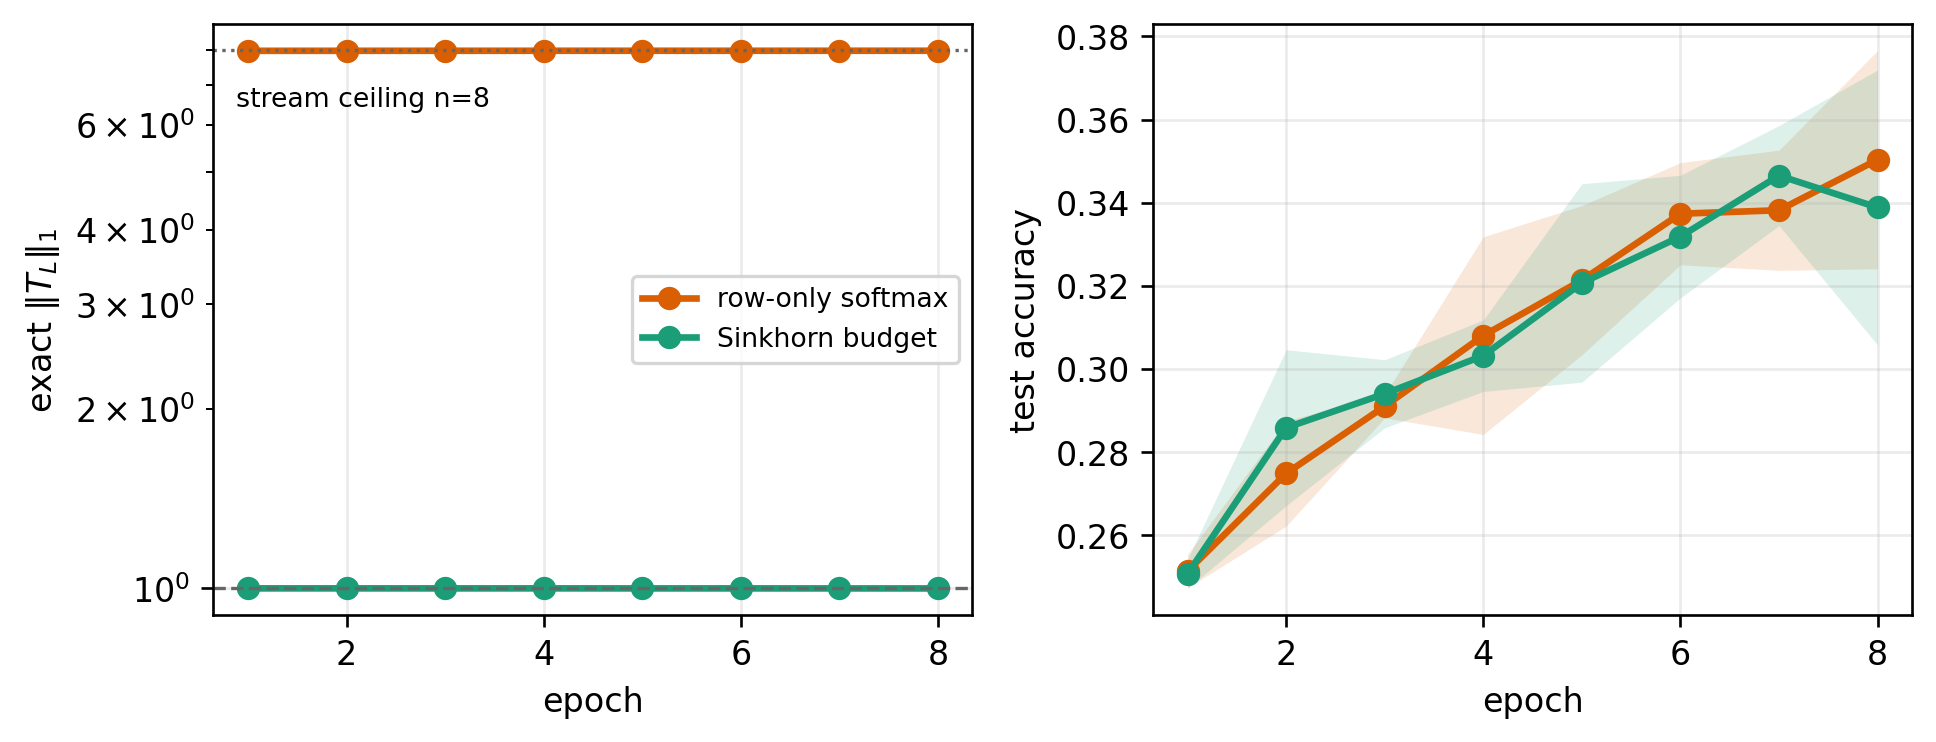
\includegraphics[width=0.88\linewidth]{tiny_transformer_relevance.png}
\caption{Matched short-horizon transformer run on a CIFAR-10 subset.
Row-only softmax mixers nearly saturate the structural backward-gain ceiling
\(n=8\), while the column-then-row Sinkhorn controller keeps the exact propagated
mixer gain near one. Test accuracy remains comparable under the same training
setup.}
\label{fig:tiny_transformer_relevance}
\end{figure}
}{%
\begin{figure}[tbp]
\centering
\fbox{\rule{0pt}{1.1in}\rule{0.82\linewidth}{0pt}}
\caption{Matched short-horizon transformer run.}
\label{fig:tiny_transformer_relevance}
\end{figure}
}

Table~\ref{tab:certificate-comparison} compares the available backward-gain
certificates on the saved final mixer stacks. For row-only softmax, the refined
Dobrushin certificate is \(7.9868\pm0.0002\), slightly sharper than the
structural ceiling \(n=8\) and close to the exact gain
\(7.9814\pm0.0036\); the product and telescoping bounds are much looser. For the
Sinkhorn-controlled stacks, the Dobrushin certificate is
\(1.000079\pm0.000009\), compared with the exact gain
\(1.000015\pm0.000002\). Among the reported bounds, the layerwise finite-horizon certificate is the smallest in both regimes.
\IfFileExists{tables/certificate_comparison_table.tex}{%
\begin{center}
\small
\setlength{\tabcolsep}{3.5pt}
\begin{tabular}{lccccc}
\toprule
Mixer policy & Product & Structural & Telescoping & Dobrushin & Exact \\
\midrule
row-only softmax & \((4.459\pm 0.001)\times 10^{21}\) & \(8\) & \(1289.47\pm 0.57\) & \(7.98679\pm 0.00015\) & \(7.9814\pm 0.0036\) \\
Sinkhorn budget & \(1.0063\pm 0.0016\) & \(8\) & \(1.0063\pm 0.0016\) & \(1.000079\pm 0.000009\) & \(1.000015\pm 0.000002\) \\
\bottomrule
\end{tabular}
\captionof{table}{Comparison of backward-gain certificates on the saved final matched-run mixer stacks. Statistics are mean$\pm$std over three seeds.}
\label{tab:certificate-comparison}
\end{center}

}{%
\begin{center}
\small
\setlength{\tabcolsep}{3.5pt}
\begin{tabular}{lrrrrr}
\toprule
Mixer policy & Product & Structural & Telescoping & Dobrushin & Exact \\
\midrule
row-only softmax & $(4.459\pm0.001)\!\times\!10^{21}$ & $8$ & $1289.47\pm0.57$ & $7.98679\pm0.00015$ & $7.9814\pm0.0036$ \\
Sinkhorn budget & $1.0063\pm0.0016$ & $8$ & $1.0063\pm0.0016$ & $1.000079\pm0.000009$ & $1.000015\pm0.000002$ \\
\bottomrule
\end{tabular}
\captionof{table}{Comparison of backward-gain certificates on the saved final
matched-run mixer stacks.}
\label{tab:certificate-comparison}
\end{center}
}

The remaining diagnostics for the matched transformer run are reported in
Appendix~\ref{app:relevance-extra}. The column-marginal errors confirm that the
Sinkhorn controller enforces the intended finite-step tolerance, while the
Dobrushin audit compares the refined finite-horizon and depth-uniform controls
on the saved final mixer stacks.

\subsection{Controller ablation and finite-step diagnostics}
The main CIFAR-10 stress setting uses \(L=128\), \(n=8\) streams, feature dimension
\(d=128\), SGD with learning rate \(0.02\), momentum \(0.9\), weight decay
\(5\times 10^{-4}\), Sinkhorn tolerance \(\varepsilon_{\mathrm{tol}}=5\times10^{-4}\),
and cap \(t_{\max}=80\). The softmax branch uses the same architecture but a
row-stochastic softmax mixer. This stress setting uses a larger mixer-logit scale
and temperature than the matched run above, making early stopping, cap failures,
and dynamic-range effects more visible.

The training run records final-epoch dynamic range, early-stopping counts, exact propagated
gain, product certificates, local spectral rates, and cap failures. Additional audit tables
and raw logs are included in the supplementary archive.

For the certificate-aware ablation, define
\[
\mathcal R_{\mathrm{budget}}
=
\left[\sum_{\ell=1}^L\log(1+\varepsilon_c^{(\ell)})-\log B_1\right]_+^2
\]
and train with
\[
\mathcal L_{\mathrm{total}}
=
\mathcal L_{\mathrm{task}}
+\lambda_{\mathrm{cert}}\mathcal R_{\mathrm{budget}}
+\lambda_\kappa\sum_{\ell=1}^L
\left[\log\kappa_\ell-\log\kappa_{\max}\right]_+^2.
\]
This is an optimization penalty rather than a substitute for certification: the hard
mixer-product bound is still evaluated from the realized post-normalization defects.

To test the controller in Lemma~\ref{lem:adaptive-budget}, we reran the same CIFAR-10
stress setting with only the Sinkhorn stopping/control policy changed.
Table~\ref{tab:focused_controller_ablation} compares fixed cap, uniform early stopping,
adaptive log-budget stopping, and an adaptive policy trained with the penalty above.

The fixed-cap policy spends substantially more Sinkhorn steps and produces a certificate
well below the prescribed budget. Uniform tolerance gives similar accuracy and exact
realized backward gain using about one fifth of the Sinkhorn iterations. The adaptive
log-budget policy spends the intended product budget more directly and slightly reduces
iterations and epoch time relative to uniform tolerance. The certificate-aware penalty
achieves similar accuracy and certified gain but incurs substantially higher training cost
in this implementation (570.2 s/epoch versus 309.6 s/epoch for adaptive stopping),
reflecting the additional differentiable certificate computation. Among the tested policies that retain a hard realized certificate, adaptive stopping has the lowest reported training cost.
\IfFileExists{paper-extra-experiments/logs/focused_controller_ablation_table.tex}{%
\begin{center}
\small
\setlength{\tabcolsep}{3pt}
\begin{tabular}{lcccccc}
\toprule
Policy & Acc. & Time/epoch & Avg. steps & Cert. & Exact $\|T_L\|_1$ & Cap fail. \\
\midrule
Fixed \(t=80\) & $0.584\pm0.037$ & $758.0\pm6.1$s & $80.00\pm0.00$ & $1.0004\pm0.0003$ & $1.00000\pm0.00000$ & $0.00\pm0.00\%$ \\
Uniform tol. & $0.584\pm0.037$ & $325.4\pm17.6$s & $16.36\pm0.71$ & $1.0521\pm0.0012$ & $1.00029\pm0.00014$ & $0.26\pm0.37\%$ \\
Adaptive budget & $0.581\pm0.034$ & $309.6\pm19.1$s & $15.86\pm0.73$ & $1.0659\pm0.0001$ & $1.00029\pm0.00014$ & $0.26\pm0.37\%$ \\
Cert.-aware penalty & $0.584\pm0.038$ & $570.2\pm34.2$s & $15.80\pm0.72$ & $1.0656\pm0.0000$ & $1.00030\pm0.00014$ & $0.26\pm0.37\%$ \\
\bottomrule
\end{tabular}
\captionof{table}{Focused controller ablation under the CIFAR-10 stress setting. The adaptive and certificate-aware policies use the shared budget $B_1=(1+5\cdot10^{-4})^{128}=1.066075$. Statistics are computed over seeds $0,1,2$; the associated local rates are all approximately $\rho_*=0.62$.}
\label{tab:focused_controller_ablation}
\end{center}

}{%
\begin{table}[tbp]
\centering
\small
\setlength{\tabcolsep}{3pt}
\caption{Focused controller ablation in the CIFAR-10 stress setting.}
\label{tab:focused_controller_ablation}
\begin{tabular}{@{}lrrrrrr@{}}
\toprule
Policy & Acc. & Time/epoch (s) & Avg. steps & Product cert. & Exact $\|T_L\|_1$ & Cap fail. \\
\midrule
Fixed cap & $0.584\pm0.037$ & $758.0\pm6.1$ & $80.00\pm0.00$ & $1.0004\pm0.0003$ & $1.00000\pm0.00000$ & $0.00\pm0.00\%$ \\
Uniform & $0.584\pm0.037$ & $325.4\pm17.6$ & $16.36\pm0.71$ & $1.0521\pm0.0012$ & $1.00029\pm0.00014$ & $0.26\pm0.37\%$ \\
Adaptive & $0.581\pm0.034$ & $309.6\pm19.1$ & $15.86\pm0.73$ & $1.0659\pm0.0001$ & $1.00029\pm0.00014$ & $0.26\pm0.37\%$ \\
Cert.-aware & $0.584\pm0.038$ & $570.2\pm34.2$ & $15.80\pm0.72$ & $1.0656\pm0.0000$ & $1.00030\pm0.00014$ & $0.26\pm0.37\%$ \\
\bottomrule
\end{tabular}
\end{table}
}

\paragraph{Sensitivity to the target budget.}
To isolate the certificate--compute trade-off from retraining, we apply the
adaptive controller post hoc to the three saved final row-only mixer stacks from
the matched transformer run, treating each positive row-stochastic mixer as the
starting matrix for column-then-row normalization. Table~\ref{tab:budget-sensitivity}
varies only \(B_1\); it does not evaluate task accuracy after renormalization.
Relaxing the budget from \(1.005\) to \(1.5\) reduces the mean full-step count
from \(2.01\) to \(1.00\) and the measured CPU normalization time from about
\(0.30\) to \(0.17\) ms per 24-layer stack.  Every realized product certificate
remains below its assigned budget, every cap-failure rate is zero, and the exact
gain remains between \(1.0000\) and \(1.0062\). At looser budgets the certificate can remain well below the assigned value because full Sinkhorn steps are discrete; \(B_1\) is only an upper bound.
\IfFileExists{tables/budget_sensitivity_table.tex}{%
\begin{center}
\small
\begin{tabular}{rrrrrr}
\toprule
Budget \(B_1\) & Avg. steps & CPU ms/stack & Product cert. & Exact \(\|T_L\|_1\) & Cap fail. \\
\midrule
1.005 & \(2.0139\pm 0.0196\) & \(0.3044\pm 0.0062\) & \(1.0013\pm 0.0002\) & \(1.0000\pm 0.0000\) & \(0\%\) \\
1.01207 & \(1.9583\pm 0.0000\) & \(0.2937\pm 0.0014\) & \(1.0063\pm 0.0017\) & \(1.0001\pm 0.0001\) & \(0\%\) \\
1.03 & \(1.8333\pm 0.0589\) & \(0.2771\pm 0.0087\) & \(1.0225\pm 0.0052\) & \(1.0001\pm 0.0001\) & \(0\%\) \\
1.06608 & \(1.6667\pm 0.0680\) & \(0.2588\pm 0.0052\) & \(1.0427\pm 0.0067\) & \(1.0001\pm 0.0001\) & \(0\%\) \\
1.1 & \(1.4444\pm 0.1094\) & \(0.2242\pm 0.0147\) & \(1.0742\pm 0.0109\) & \(1.0001\pm 0.0001\) & \(0\%\) \\
1.25 & \(1.0556\pm 0.0520\) & \(0.1754\pm 0.0070\) & \(1.1584\pm 0.0101\) & \(1.0038\pm 0.0025\) & \(0\%\) \\
1.5 & \(1.0000\pm 0.0000\) & \(0.1647\pm 0.0003\) & \(1.1776\pm 0.0284\) & \(1.0061\pm 0.0008\) & \(0\%\) \\
\bottomrule
\end{tabular}
\captionof{table}{Post-hoc global-budget sensitivity on saved final matched-run mixer stacks. Timing is for normalization of one 24-layer stack on a single CPU process and excludes file loading. Statistics are mean$\pm$std over three seeds.}
\label{tab:budget-sensitivity}
\end{center}

}{%
\begin{center}
\small
\setlength{\tabcolsep}{4pt}
\begin{tabular}{rrrrrr}
\toprule
Budget \(B_1\) & Avg. steps & CPU ms/stack & Product cert. &
Exact \(\|T_L\|_1\) & Cap fail. \\
\midrule
$1.005$ & $2.0139\pm0.0196$ & $0.3044\pm0.0062$ & $1.0013\pm0.0002$ & $1.0000\pm0.0000$ & $0\%$ \\
$1.01207$ & $1.9583\pm0.0000$ & $0.2937\pm0.0014$ & $1.0063\pm0.0017$ & $1.0001\pm0.0001$ & $0\%$ \\
$1.03$ & $1.8333\pm0.0589$ & $0.2771\pm0.0087$ & $1.0225\pm0.0052$ & $1.0001\pm0.0001$ & $0\%$ \\
$1.06608$ & $1.6667\pm0.0680$ & $0.2588\pm0.0052$ & $1.0427\pm0.0067$ & $1.0001\pm0.0001$ & $0\%$ \\
$1.1$ & $1.4444\pm0.1094$ & $0.2242\pm0.0147$ & $1.0742\pm0.0109$ & $1.0001\pm0.0001$ & $0\%$ \\
$1.25$ & $1.0556\pm0.0520$ & $0.1754\pm0.0070$ & $1.1584\pm0.0101$ & $1.0038\pm0.0025$ & $0\%$ \\
$1.5$ & $1.0000\pm0.0000$ & $0.1647\pm0.0003$ & $1.1776\pm0.0284$ & $1.0061\pm0.0008$ & $0\%$ \\
\bottomrule
\end{tabular}
\captionof{table}{Post-hoc global-budget sensitivity on saved final matched-run
mixer stacks.}
\label{tab:budget-sensitivity}
\end{center}
}

\subsection{Calibration and local-predictor diagnostics}
Figure~\ref{fig:temperature_clipping_grid}
tests the design inequality \eqref{eq:beta-R-cert} on random clipped logit matrices with
\(n=8\). The measured column errors are always below the finite-precision certificate
when the certificate is above the numerical floor. The grid also shows why the
temperature--clipping rule is a conservative design certificate rather than a
predictor: for large \(\beta R\), the worst-case certificate is nearly vacuous
even though the measured errors decrease rapidly with \(t_{\max}\).

\begin{center}
\centering
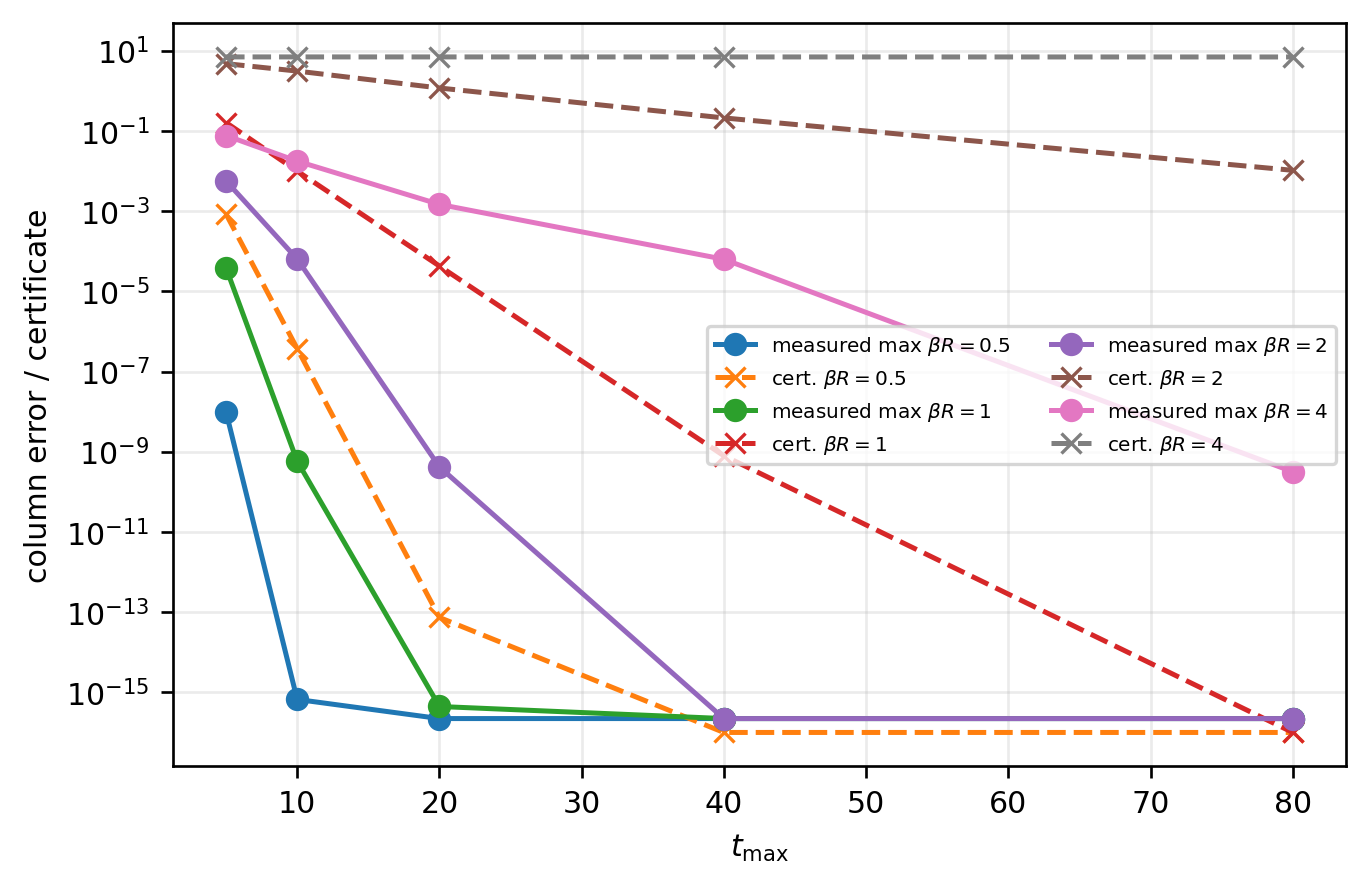
\includegraphics[width=0.72\linewidth]{temperature_clipping_grid.png}
\captionof{figure}{Temperature--clipping diagnostic for the conservative design rule
\eqref{eq:beta-R-cert}. Solid curves are measured maximum column errors over random
clipped logits; dashed curves are the corresponding worst-case certificates.}
\label{fig:temperature_clipping_grid}
\end{center}

For each Sinkhorn layer, we compute the fixed-\(t_{\max}\) matrix
\(A^{\mathrm{fix}}\), use it as the realized doubly stochastic approximation
\(P\), and report \(\rho_\ast=\sigma_2(P)^2\). We also report the empirical final-step ratio
\(\varepsilon_c^{(2t+2)}/\varepsilon_c^{(2t)}\) when the denominator is numerically
meaningful. This ratio is diagnostic only; near the early-stopping tolerance or
numerical floor it need not estimate the asymptotic local rate.

For trained adaptive Sinkhorn layers, the local first- and second-order predictors track
the measured column-error decay much more closely than the global Hilbert certificates.
The Hilbert bounds remain conservative, while the local expansions follow the
measured decay. Figure~\ref{fig:local_predictor_curve} shows a representative
trained layer.

\begin{center}
\centering
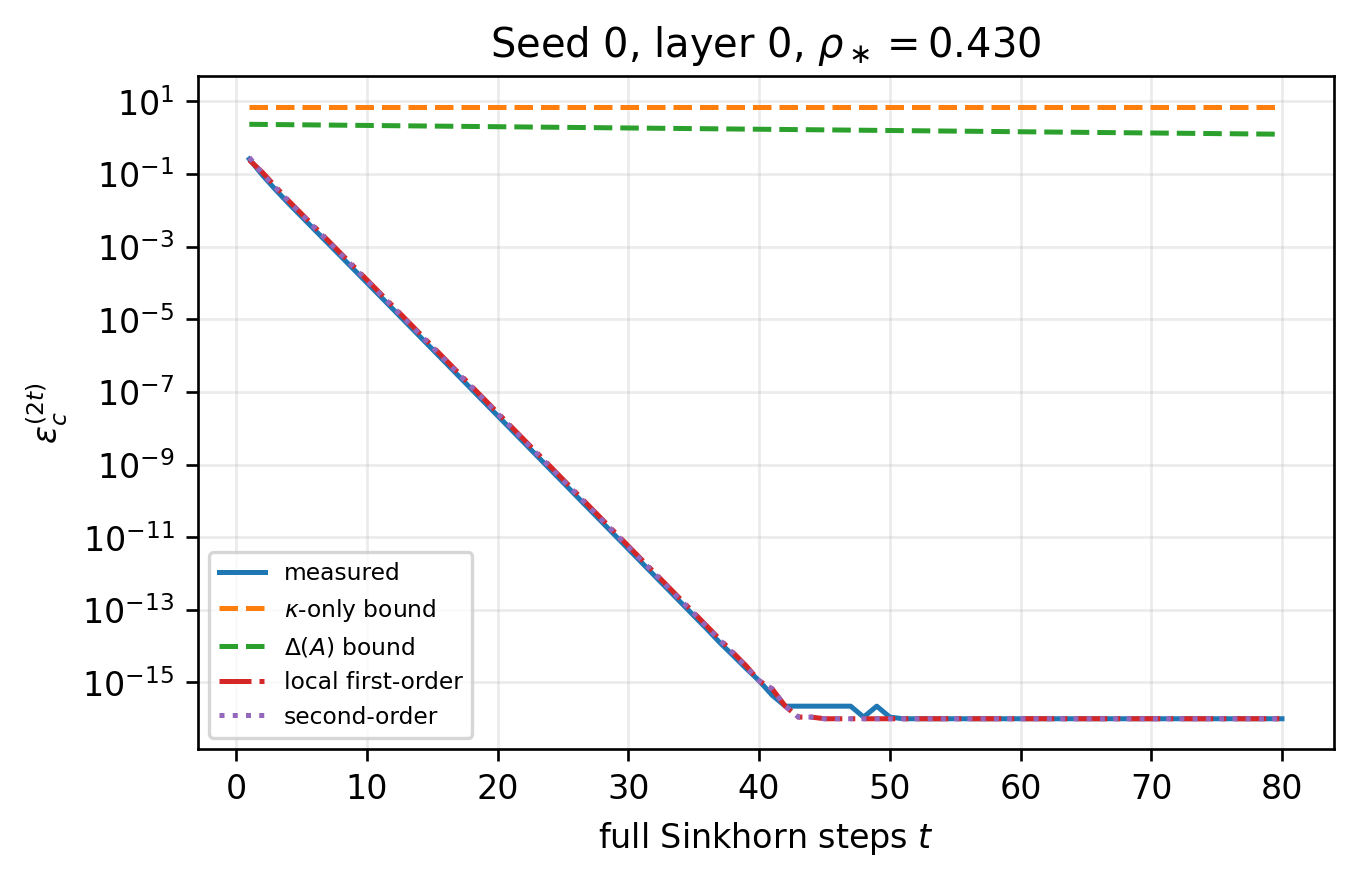
\includegraphics[width=0.72\linewidth]{local_predictor_seed0_layer0.png}
\captionof{figure}{Representative local-predictor comparison on a trained adaptive Sinkhorn layer.
The local first- and second-order predictors track the measured Sinkhorn decay closely,
while the Hilbert certificates remain conservative.}
\label{fig:local_predictor_curve}
\end{center}

The stress run operates in a high-dynamic-range regime; the corresponding
final-epoch dynamic-range audit is reported in
Appendix~\ref{app:certificate-evaluation}.

Appendix~\ref{app:extra-diagnostics} contains a compact stress-run audit figure computed
from the same logs.
\FloatBarrier

\section{Discussion and practical guidance}\label{sec:discussion}
\subsection{Practical guidance}\label{subsec:guidance}
The certificates are most informative when the desired backward mixer-path budget
lies below the structural ceiling \(n\). For nonnegative row-stochastic mixers,
\(\|T_L\|_1\le n\) independently of depth and of the Sinkhorn schedule. Measured
column defects provide the multiplicative certificate, while the telescoping bound
can sharpen it by incorporating realized prefix gains. When the mixers are uniformly
scrambling, the Dobrushin estimate gives a complementary depth-uniform audit. In the
matched row-only run, its finite-horizon value is only slightly below the structural
ceiling; for the Sinkhorn-controlled mixers it is close to one.

For a target \(B_1<n\), the small-error relation
\(\sum_{\ell=1}^L\varepsilon_c^{(\ell)}\approx\log B_1\) gives a useful scale for
allocating layerwise tolerances. Theorem~\ref{thm:calibration} converts those
tolerances into conservative requirements on \((\kappa,t_{\max})\), or equivalently
on temperature, clipping, and the step cap. The sensitivity study in
Table~\ref{tab:budget-sensitivity} shows the corresponding compute trade-off directly:
tighter budgets require more normalization work, while the realized exact gain can
remain much smaller than the certificate.

The global Hilbert estimate should be read as a design certificate rather than a
prediction of the observed convergence rate. Matrix-specific spectral quantities and
the first- and second-order expansions are useful diagnostics once a realized matrix
is available. Adaptive stopping uses measured marginal errors to reduce computation,
and Equation~\eqref{eq:exact-backward-gain} gives the exact realized backward gain
without forming the full product.

\subsection{Limitations}\label{subsec:limitations}

\noindent\textbf{Worst-case and finite-step bounds.}
The product and Hilbert-metric bounds are sufficient worst-case certificates and
can be conservative. The structural ceiling, telescoping refinement,
matrix-specific local analysis, and exact propagated gain provide
progressively more realized information when the corresponding quantities are
available. The local spectral and second-order formulas describe finite-step
decay near the Sinkhorn limit; they are predictors, not uniform certificates.

\noindent\textbf{Nonlinear blocks and training dynamics.}
The nonlinear block $F$ enters only through Jacobian norm bounds such as Proposition~\ref{prop:full-jac} and Corollary~\ref{cor:jacobian-cert}. We do not model how training shapes $\widetilde{\Hres}^{(\ell)}$ or how the certificates interact with optimization, data distribution, or generalization.

\noindent\textbf{Architecture and implementation.}
The statements use streams-as-rows and the column--then--row Sinkhorn order. Streams-as-columns, damping, mixed precision, sparse mixers, and masked supports require explicit translation and can change which marginal error remains at the output.
Exact doubly stochastic parameterizations such as mHC-lite avoid finite-step
marginal error altogether; the present calibration is relevant when iterative
Sinkhorn normalization is retained. We compare these approaches conceptually but
do not benchmark exact parameterizations against iterative Sinkhorn in this study.

\subsection{Future work}\label{subsec:future_work}
Open directions include inexpensive certification of the local derivative
envelopes in Appendix~\ref{app:local-envelope}, sharper support- or gap-dependent
refinements of the Dobrushin certificate, broader controller and
certificate-penalty ablations across datasets and architectures, and
full-network bounds that couple mixer certificates to nonlinear-branch Jacobians.


\section{Conclusion}\label{sec:conclusion}

We developed deterministic finite-step bounds for nonnegative
Sinkhorn-normalized stream mixers. Marginal errors translate directly into
forward and backward induced-norm control, while Hilbert-projective contraction
connects logit dynamic range and Sinkhorn step count to a depth-wise mixer
budget. The structural ceiling $\|T_L\|_1\le n$ and the telescoping refinement
provide complementary worst-case and realized controls, while the matrix-specific
local analysis describes the observed Sinkhorn convergence rate near the limit.

The same framework gives practical calibration and adaptive stopping rules. In
the focused ablations, adaptive log-budget stopping reaches the same mixer-path
targets as a uniform tolerance while using fewer Sinkhorn steps, whereas the
certificate-aware penalty is more expensive in the present implementation. In
the matched transformer diagnostic, Sinkhorn normalization reduces the exact
backward mixer gain from near the structural ceiling to near one while
maintaining comparable short-horizon task performance.


\section*{Reproducibility Statement}
The supplementary archive contains the scripts, fixed seeds, raw CSV/JSON logs,
figure-generation scripts, and command manifest needed to regenerate the reported
diagnostics and finite-step lookup table. Because the certificates depend on implementation
details, the archive records the Sinkhorn dtype, positivity floor
\(\varepsilon_{\mathrm{floor}}\), clipping/temperature settings, early-stopping tolerance,
data path, and preprocessing. The accompanying code is available at
\url{https://github.com/MaKosmakov/finite-step-sinkhorn-certificates}.
The supplementary archive also includes
saved final mixer stacks for the matched transformer run
and the script \texttt{scripts/dobrushin\_diagnostic.py}, which regenerates the
depth-uniform Dobrushin audit and certificate-comparison tables. The script
\texttt{scripts/budget\_sensitivity\_diagnostic.py} regenerates the post-hoc
global-budget sensitivity table from the same saved stacks.

\section*{Ethics and Broader Impact Statement}
This work studies finite-step normalization for nonnegative mixer products. The diagnostics
use CIFAR-10 and do not involve human-subject data, personal data, or deployment decisions.



\begin{thebibliography}{99}

\bibitem[Birkhoff(1957)]{Birkhoff1957}
G.~Birkhoff.
\newblock Extensions of Jentzsch's theorem.
\newblock \emph{Transactions of the American Mathematical Society}, 85:219--227, 1957.

\bibitem[Bushell(1973)]{Bushell1973}
P.~J.~Bushell.
\newblock Hilbert's metric and positive contraction mappings in a Banach space.
\newblock \emph{Archive for Rational Mechanics and Analysis}, 52:330--338, 1973.

\bibitem[He et~al.(2016)]{He2016ResNet}
K.~He, X.~Zhang, S.~Ren, and J.~Sun.
\newblock Deep residual learning for image recognition.
\newblock In \emph{Proceedings of the IEEE Conference on Computer Vision and Pattern Recognition}, 2016.

\bibitem[Vaswani et~al.(2017)]{Vaswani2017Attention}
A.~Vaswani, N.~Shazeer, N.~Parmar, et~al.
\newblock Attention is all you need.
\newblock In \emph{Advances in Neural Information Processing Systems}, 2017.

\bibitem[Xie et~al.(2025)]{Xie2025mHC}
Z.~Xie, Y.~Wei, H.~Cao, et~al.
\newblock {mHC: Manifold-Constrained Hyper-Connections}.
\newblock \emph{arXiv preprint arXiv:2512.24880}, 2025.
\newblock DOI: 10.48550/arXiv.2512.24880.
\newblock \url{https://arxiv.org/abs/2512.24880}.

\bibitem[Yang and Gao(2026)]{YangGao2026mHCLite}
Y.~Yang and J.~Gao.
\newblock {mHC-lite: You Don't Need 20 Sinkhorn--Knopp Iterations}.
\newblock \emph{arXiv preprint arXiv:2601.05732}, 2026.
\newblock DOI: 10.48550/arXiv.2601.05732.
\newblock \url{https://arxiv.org/abs/2601.05732}.


\bibitem[Sinkhorn and Knopp(1967)]{SinkhornKnopp1967}
R.~Sinkhorn and P.~Knopp.
\newblock Concerning nonnegative matrices and doubly stochastic matrices.
\newblock \emph{Pacific Journal of Mathematics}, 21:343--348, 1967.

\bibitem[Franklin and Lorenz(1989)]{FranklinLorenz1989}
J.~Franklin and J.~Lorenz.
\newblock On the scaling of multidimensional matrices.
\newblock \emph{Linear Algebra and its Applications}, 114--115:717--735, 1989.

\bibitem[Knight(2008)]{Knight2008}
P.~A.~Knight.
\newblock The Sinkhorn--Knopp algorithm: convergence and applications.
\newblock \emph{SIAM Journal on Matrix Analysis and Applications}, 30(1):261--275, 2008.


\bibitem[Cuturi(2013)]{Cuturi2013}
M.~Cuturi.
\newblock Sinkhorn distances: light-speed computation of optimal transport.
\newblock In \emph{Advances in Neural Information Processing Systems (NeurIPS)}, 2013.

\bibitem[Peyr\'e and Cuturi(2019)]{PeyreCuturi2019}
G.~Peyr\'e and M.~Cuturi.
\newblock \emph{Computational Optimal Transport}.
\newblock Foundations and Trends in Machine Learning, 11:355--607, 2019.

\bibitem[Sander et~al.(2022)]{Sander2022Sinkformers}
M.~E.~Sander, P.~Ablin, M.~Blondel, and G.~Peyr\'e.
\newblock Sinkformers: Transformers with Doubly Stochastic Attention.
\newblock In \emph{Proceedings of AISTATS 2022}, PMLR 151, 2022.
\newblock arXiv:2110.11773.

\bibitem[Shahbazi et~al.(2025)]{Shahbazi2025ESPFormer}
A.~Shahbazi, E.~Akbari, D.~Salehi, X.~Liu, N.~NaderiAlizadeh, and S.~Kolouri.
\newblock ESPFormer: Doubly-Stochastic Attention with Expected Sliced Transport Plans.
\newblock In \emph{Proceedings of the 42nd International Conference on Machine Learning},
PMLR 267:54186--54202, 2025.


\bibitem[Haber and Ruthotto(2018)]{HaberRuthotto2018}
E.~Haber and L.~Ruthotto.
\newblock Stable architectures for deep neural networks.
\newblock \emph{Inverse Problems}, 34:014004, 2018.

\bibitem[Chen et~al.(2018)]{Chen2018NeuralODE}
R.~T.~Q.~Chen, Y.~Rubanova, J.~Bettencourt, and D.~K.~Duvenaud.
\newblock Neural ordinary differential equations.
\newblock In \emph{Advances in Neural Information Processing Systems (NeurIPS)}, 2018.


\end{thebibliography}

\appendix

\renewcommand{\thetable}{A.\arabic{table}}
\setcounter{table}{0}
\renewcommand{\theHtable}{appendix.A.\arabic{table}}
\renewcommand{\thefigure}{A.\arabic{figure}}
\setcounter{figure}{0}
\renewcommand{\theHfigure}{appendix.A.\arabic{figure}}


\section{Certificate evaluation and additional diagnostics}
\label{app:certificate-evaluation}

For each layer, the implementation computes
\(\bar\varepsilon_\ell
=\exp((\log B_1-\sum_{j<\ell}\log(1+\varepsilon_c^{(j)}))/(L-\ell+1))-1\)
and runs column-then-row Sinkhorn steps until either
\(\varepsilon_c^{(\ell)}(t)=
\|\ones^\top S^{(2t)}-\ones^\top\|_{\infty,\mathrm{vec}}
\le \bar\varepsilon_\ell\) or \(t=t_{\max}\). The reported product
certificate is \(\exp(\sum_{\ell=1}^L\log(1+\varepsilon_c^{(\ell)}))\), and
the exact realized backward gain is computed by the recursion \(w_L=\ones\),
\(w_{\ell-1}=(\Hres^{(\ell)})^\top w_\ell\), and
\(\|T_L\|_1=\|w_0\|_{\infty,\mathrm{vec}}\).
If any layer reaches \(t_{\max}\) before satisfying its assigned tolerance, the adaptive
budget certificate is marked as failed.

This appendix collects post-hoc certificate diagnostics and the stress-run audit plots.

\subsection{Finite-horizon and depth-uniform Dobrushin diagnostic}
\label{app:dobrushin-diagnostic}

To audit Proposition~\ref{prop:ergodic} on trained mixers, we saved the final
per-layer residual mixer stacks from the matched transformer run and computed the
finite-horizon Dobrushin certificate
\[
1+\frac12\sum_{\ell=1}^L
\left(\prod_{j=1}^{\ell-1}\delta_j\right)
\|c_\ell\|_{1,\mathrm{vec}},
\]
where
\(c_\ell=(H^{(\ell)})^\top\ones-\ones\) and
\(\delta_\ell=\delta_{\mathrm D}(H^{(\ell)})\). The corresponding
depth-uniform bound follows by replacing the layerwise quantities by their
maxima as in \eqref{eq:dobrushin-uniform-cert}.
The diagnostic uses the same final matched-run setting as
Figure~\ref{fig:tiny_transformer_relevance}: three seeds, \(5000\) training
images, \(2000\) test images, eight epochs, depth \(L=24\), and \(n=8\) streams.

\IfFileExists{tables/dobrushin_diagnostic_table.tex}{%
\begin{center}
\centering
\small
\begin{tabular}{lrrrrrrr}
\toprule
Policy & \(L\) & \(n\) & \(\bar\delta\) & \(\max_\ell\|c_\ell\|_1\) & Product cert. & Dobrushin cert. & Exact \(\|T_L\|_1\) \\
\midrule
softmax seed 0 & 24 & 8 & \(9.267\times 10^{-4}\) & \(13.96\) & \(4.457\times 10^{21}\) & \(7.987\) & \(7.976\) \\
sinkhorn seed 0 & 24 & 8 & \(0.2345\) & \(0.01692\) & \(1.0086\) & \(1.0001\) & \(1.0000\) \\
softmax seed 1 & 24 & 8 & \(7.792\times 10^{-4}\) & \(13.96\) & \(4.460\times 10^{21}\) & \(7.987\) & \(7.985\) \\
sinkhorn seed 1 & 24 & 8 & \(0.2082\) & \(0.01364\) & \(1.0053\) & \(1.0001\) & \(1.0000\) \\
softmax seed 2 & 24 & 8 & \(9.942\times 10^{-4}\) & \(13.96\) & \(4.460\times 10^{21}\) & \(7.987\) & \(7.983\) \\
sinkhorn seed 2 & 24 & 8 & \(0.2006\) & \(0.01372\) & \(1.0050\) & \(1.0001\) & \(1.0000\) \\
\bottomrule
\end{tabular}
\captionof{table}{Post-hoc finite-horizon Dobrushin diagnostics for saved mixer stacks.}
\label{tab:dobrushin-diagnostic}
\end{center}

}{%
\begin{table}[tbp]
\centering
\small
\setlength{\tabcolsep}{3pt}
\caption{Finite-horizon Dobrushin diagnostic on saved final matched-run mixers.}
\label{tab:dobrushin-diagnostic}
\begin{tabular}{lrrrrrrr}
\toprule
Policy & Seed & $L$ & $n$ & $\max\delta_\ell$ & $\max\|c_\ell\|_1$ & Dobrushin cert. & Exact $\|T_L\|_1$ \\
\midrule
softmax & 0 & 24 & 8 & $9.267\times10^{-4}$ & $13.96$ & $7.987$ & $7.976$ \\
sinkhorn & 0 & 24 & 8 & $0.2345$ & $0.01692$ & $1.0001$ & $1.0000$ \\
softmax & 1 & 24 & 8 & $7.792\times10^{-4}$ & $13.96$ & $7.987$ & $7.985$ \\
sinkhorn & 1 & 24 & 8 & $0.2082$ & $0.01364$ & $1.0001$ & $1.0000$ \\
softmax & 2 & 24 & 8 & $9.942\times10^{-4}$ & $13.96$ & $7.987$ & $7.983$ \\
sinkhorn & 2 & 24 & 8 & $0.2006$ & $0.01372$ & $1.0001$ & $1.0000$ \\
\bottomrule
\end{tabular}
\end{table}
}

For the Sinkhorn-controlled mixers, the refined Dobrushin certificate is near
one and close to the exact propagated gain. For the row-only softmax mixers, it
is slightly smaller than the structural ceiling and again close to the exact
gain. The product certificate remains the controller's directly allocated
budget; the post-hoc Dobrushin calculation is the smallest reported audit bound
for these saved stacks.
\FloatBarrier

\subsection{Additional matched-run diagnostics}
\label{app:relevance-extra}

The remaining matched-run diagnostics are shown in
Figure~\ref{fig:relevance-extra}. The column-error panel records the finite-step marginal defect, and the
gradient-norm panel is included as an auxiliary training diagnostic.

\IfFileExists{relevance-demo/plots/tiny_transformer_relevance_extra.png}{%
\begin{center}
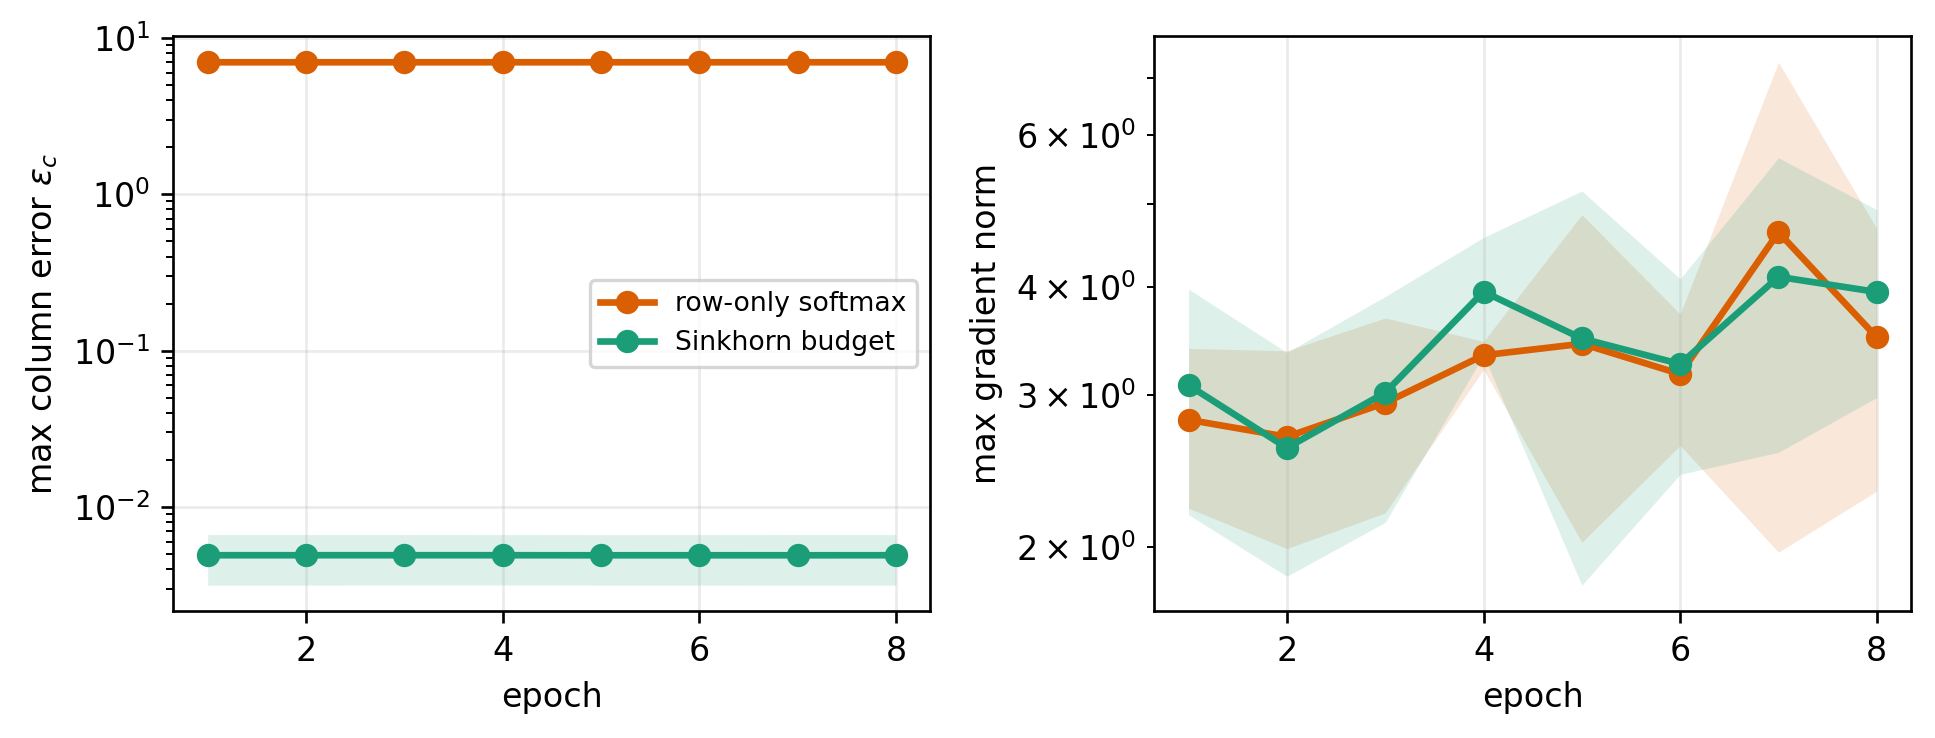
\includegraphics[width=0.88\linewidth]{tiny_transformer_relevance_extra.png}
\captionof{figure}{Additional matched-run diagnostics. The column-error panel
records the finite-step marginal defect, and the gradient-norm panel is included
as an implementation audit.}
\label{fig:relevance-extra}
\end{center}
}{%
\begin{figure}[tbp]
\centering
\fbox{\rule{0pt}{1.1in}\rule{0.82\linewidth}{0pt}}
\caption{Additional matched-run diagnostics.}
\label{fig:relevance-extra}
\end{figure}
}
\FloatBarrier

\subsection{Stress-run audit}
\label{app:extra-diagnostics}

These diagnostics use the same stress-run logs as the main certificate tables.

\IfFileExists{results-stressed-cap80/logs/kappa_tstop_table.tex}{%
\paragraph{Dynamic-range audit.}
Table~\ref{tab:appendix-dynamic-range} reports the final-epoch dynamic-range
diagnostics for the stress run. For Sinkhorn, the fixed-cap column evaluates the
same trained weights using \(t=t_{\max}\). For the row-softmax baseline,
\(\kappa_{\mathrm{obs}}\) is a native pre-softmax diagnostic, not the clipped
positive-matrix dynamic range used in the Sinkhorn certificate.

\begin{center}
\centering
\small
\captionof{table}{Final-epoch dynamic-range diagnostics for the stress run.}
\label{tab:appendix-dynamic-range}
\begin{tabular}{lcccc}
\toprule
Model & med. $\kappa_{\mathrm{obs}}$ & std & med. $\kappa_{\mathrm{obs}}^{\mathrm{fix}}$ & std \\
\midrule
softmax & 8556629.04 & 840682.39 & --- & --- \\
sinkhorn (early) & 14489.91 & 1315.73 & 14487.00 & 1324.17 \\
\bottomrule
\end{tabular}
\end{center}

\begin{center}
\centering
\small
\captionof{table}{Final-epoch stack certificate diagnostics. The exact backward gain is computed
by vector propagation, while the certificate is
\(\prod_{\ell}(1+\varepsilon_c^{(\ell)})\).}
\label{tab:stack_certificate_diag}
\begin{tabular}{lccc}
\toprule
Model & cert. & exact $\|T_L\|_1$ & exact/cert. \\
\midrule
softmax & \(3.61{\times}10^{47}\pm5{\times}10^{47}\) & \(5.72\pm2\) & --- \\
sinkhorn (early) & \(1.05\pm0.0009\) & \(1\pm8{\times}10^{-5}\) & \(0.951\pm0.0009\) \\
\bottomrule
\end{tabular}
\end{center}
\FloatBarrier

\noindent For the early-stopped Sinkhorn run, the final epoch reaches the tolerance
\(\varepsilon_{\mathrm{tol}}=5\times 10^{-4}\) with median stopping time
\(t_{\mathrm{stop}}=14\). Re-evaluating the same trained weights with the full cap
\(t_{\max}=80\) gives a smaller column defect, about \(1.9\times 10^{-4}\), confirming
that the reported stopping behavior is tolerance-driven rather than cap-limited.

The row-softmax baseline illustrates that row stochasticity alone does not give a useful
backward product certificate: the product certificate is enormous, although the realized
gain is structurally capped and remains \(O(n)\). The Sinkhorn controller keeps both the
certificate and the exact propagated gain near one.

For the Sinkhorn run, the associated local diagnostic is
\(\rho_\ast=0.631\pm0.01\), and the cap-failure rate is zero.
\FloatBarrier

}{%
\paragraph{Dynamic-range audit.}
Table~\ref{tab:kappa-stress} reports final-epoch dynamic-range diagnostics for the
stress run. For Sinkhorn, the fixed-cap column evaluates the same trained weights
using \(t=t_{\max}\). For the row-softmax baseline, \(\kappa_{\mathrm{obs}}\) is a
native pre-softmax diagnostic, not the clipped positive-matrix dynamic range used
in the Sinkhorn certificate.

\begin{table}[tbp]
\centering
\small
\caption{Final-epoch dynamic-range diagnostics for the stress run.}
\label{tab:kappa-stress}
\begin{tabular}{lrrrr}
\toprule
Model & med. $\kappa_{\mathrm{obs}}$ & std & med. $\kappa_{\mathrm{obs}}^{\mathrm{fix}}$ & std \\
\midrule
softmax & $8556629.04$ & $840682.39$ & --- & --- \\
sinkhorn (early) & $14489.91$ & $1315.73$ & $14487.00$ & $1324.17$ \\
\bottomrule
\end{tabular}
\end{table}

\begin{table}[tbp]
\centering
\small
\caption{Final-epoch stack certificate diagnostics. The exact backward gain is
computed by vector propagation; the product certificate is
$\prod_\ell(1+\varepsilon_c^{(\ell)})$.}
\label{tab:stack-cert-stress}
\begin{tabular}{lrrr}
\toprule
Model & Product cert. & Exact $\|T_L\|_1$ & Exact/cert. \\
\midrule
softmax & $(3.61\pm5.00)\times10^{47}$ & $5.72\pm2.00$ & --- \\
sinkhorn (early) & $1.0500\pm0.0009$ & $1.0000\pm8\times10^{-5}$ & $0.951\pm0.0009$ \\
\bottomrule
\end{tabular}
\end{table}

For the early-stopped Sinkhorn run, the final epoch reaches the tolerance
\(\varepsilon_{\mathrm{tol}}=5\times10^{-4}\) with median stopping time
\(t_{\mathrm{stop}}=14\). Re-evaluating the same trained weights at
\(t_{\max}=80\) gives a column defect of about \(1.9\times10^{-4}\). The associated
local diagnostic is \(\rho_*=0.631\pm0.01\), and no layer reaches the step cap
without satisfying its tolerance. For the row-softmax baseline, the product
certificate is very large while the realized gain remains bounded by the
row-stochastic structural ceiling.
}

\paragraph{Stress-run audit trajectories.}
Figure~\ref{fig:stress-audit} summarizes the main stress-run diagnostics over
training. The maximum column defect stays near the early-stopping tolerance, the
product certificate remains below the prescribed budget, and the exact propagated
gain stays close to one. The stopping-count panel records the compute savings from
early stopping. Cap failures are zero in the reported run.

\begin{center}
\begin{minipage}{0.49\linewidth}
\centering
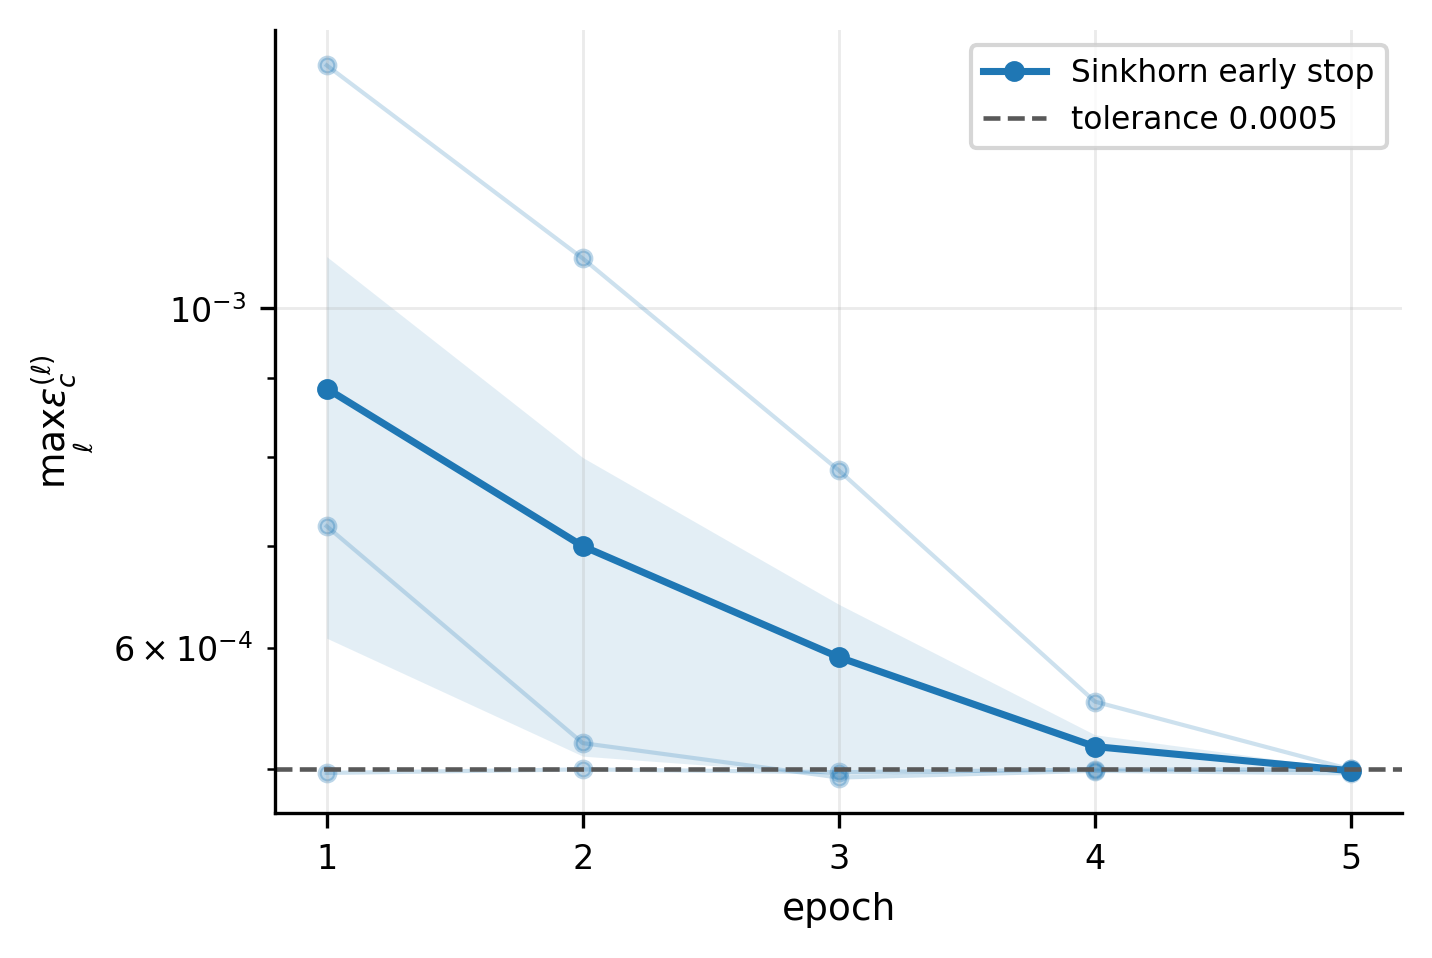
\includegraphics[width=\linewidth]{max_eps_c.png}
\small (a) Maximum column defect.
\end{minipage}\hfill
\begin{minipage}{0.49\linewidth}
\centering
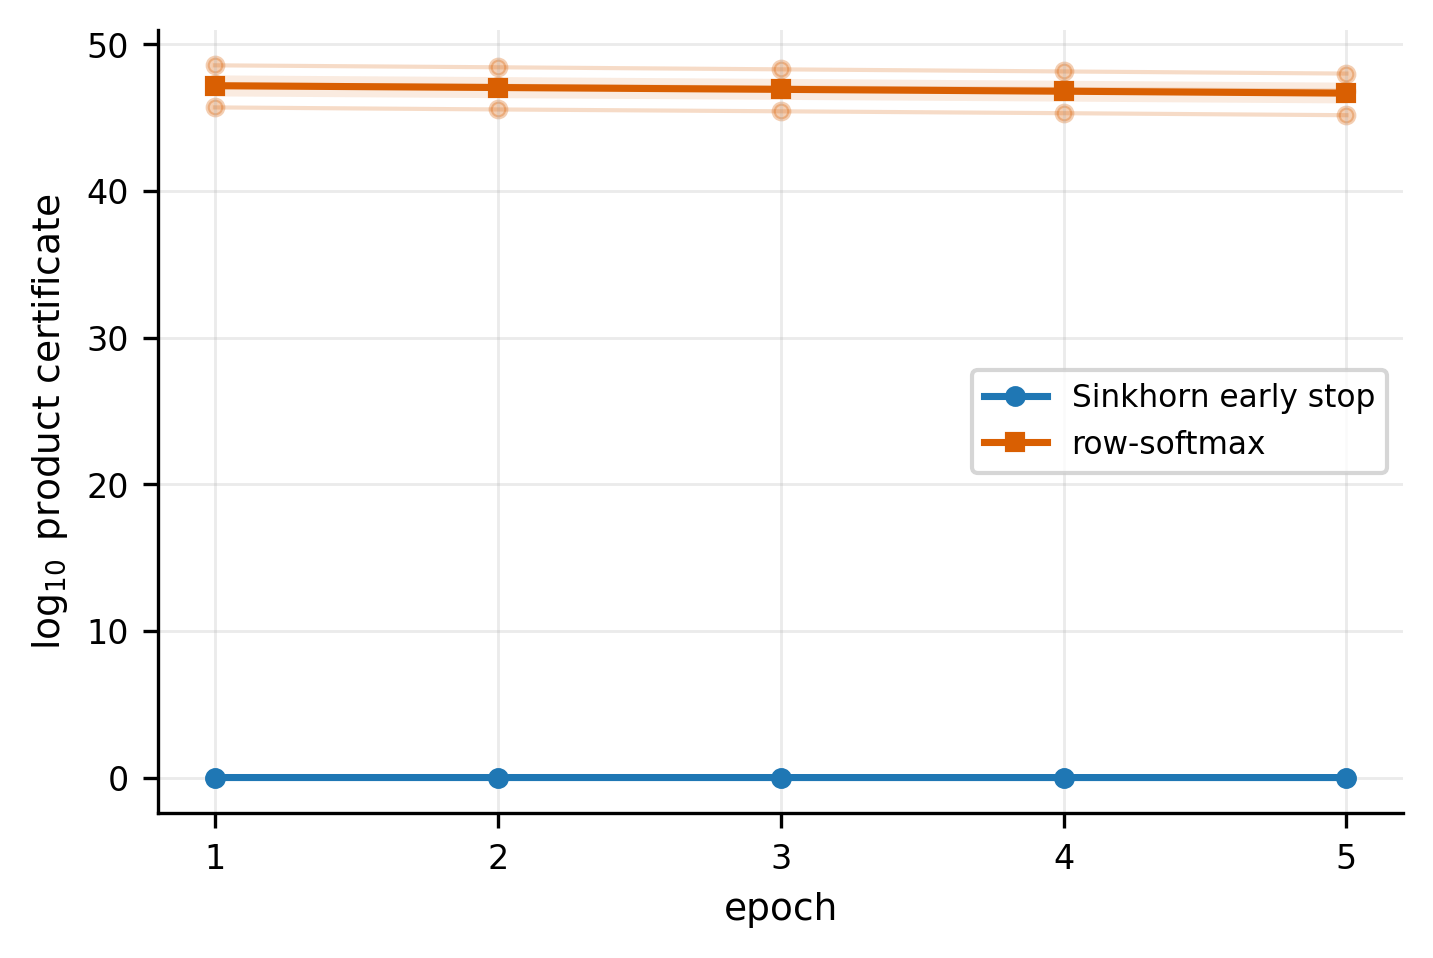
\includegraphics[width=\linewidth]{cert_bound.png}
\small (b) Product certificate.
\end{minipage}

\medskip
\begin{minipage}{0.49\linewidth}
\centering
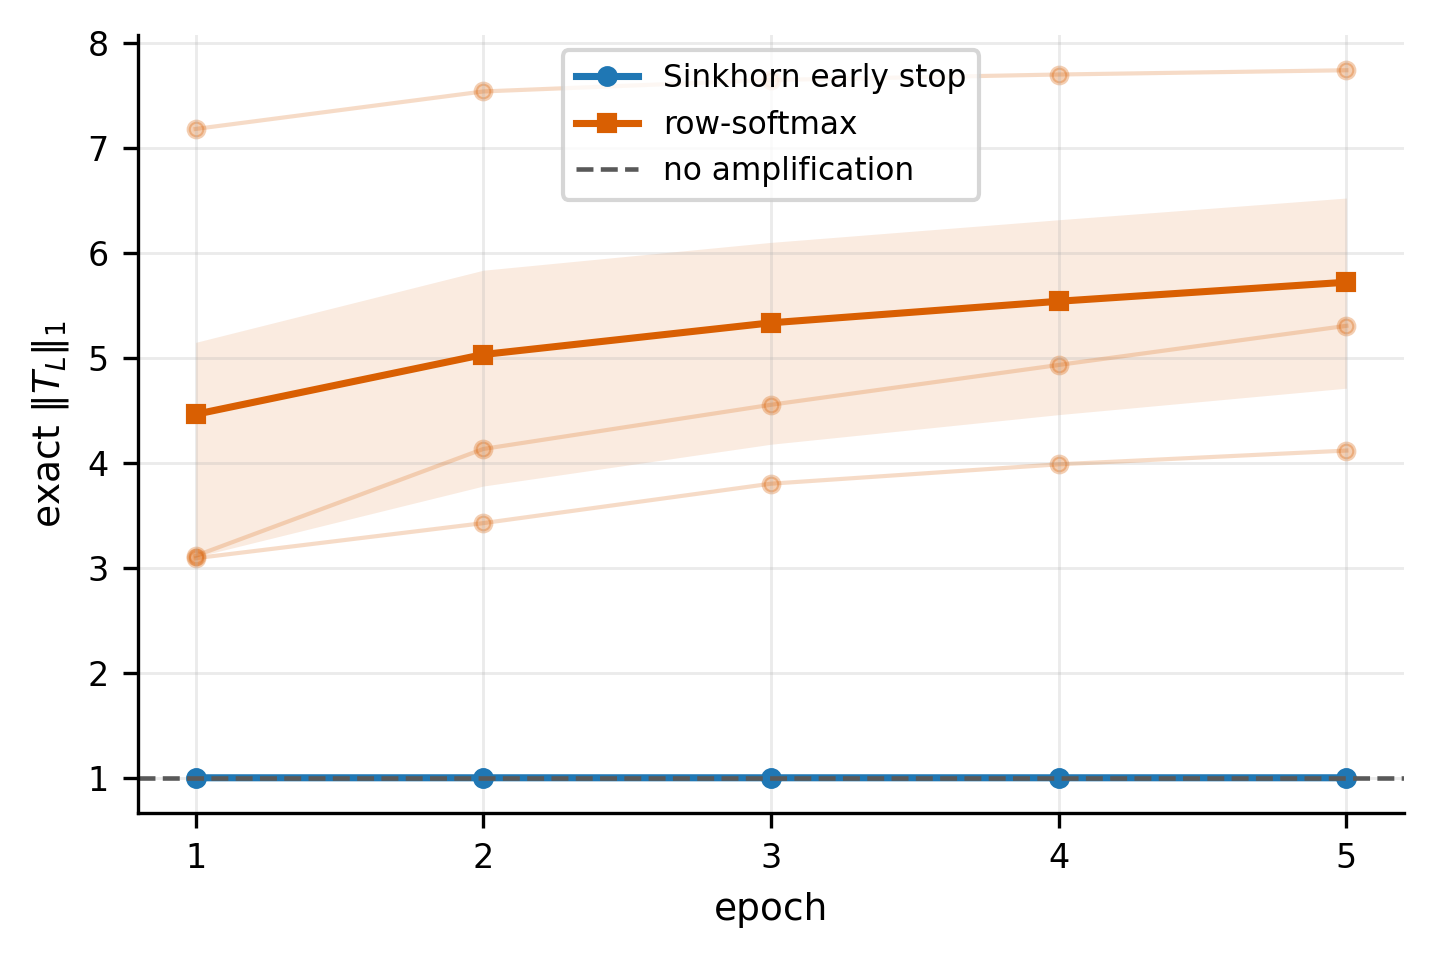
\includegraphics[width=\linewidth]{exact_T1.png}
\small (c) Exact propagated gain.
\end{minipage}\hfill
\begin{minipage}{0.49\linewidth}
\centering
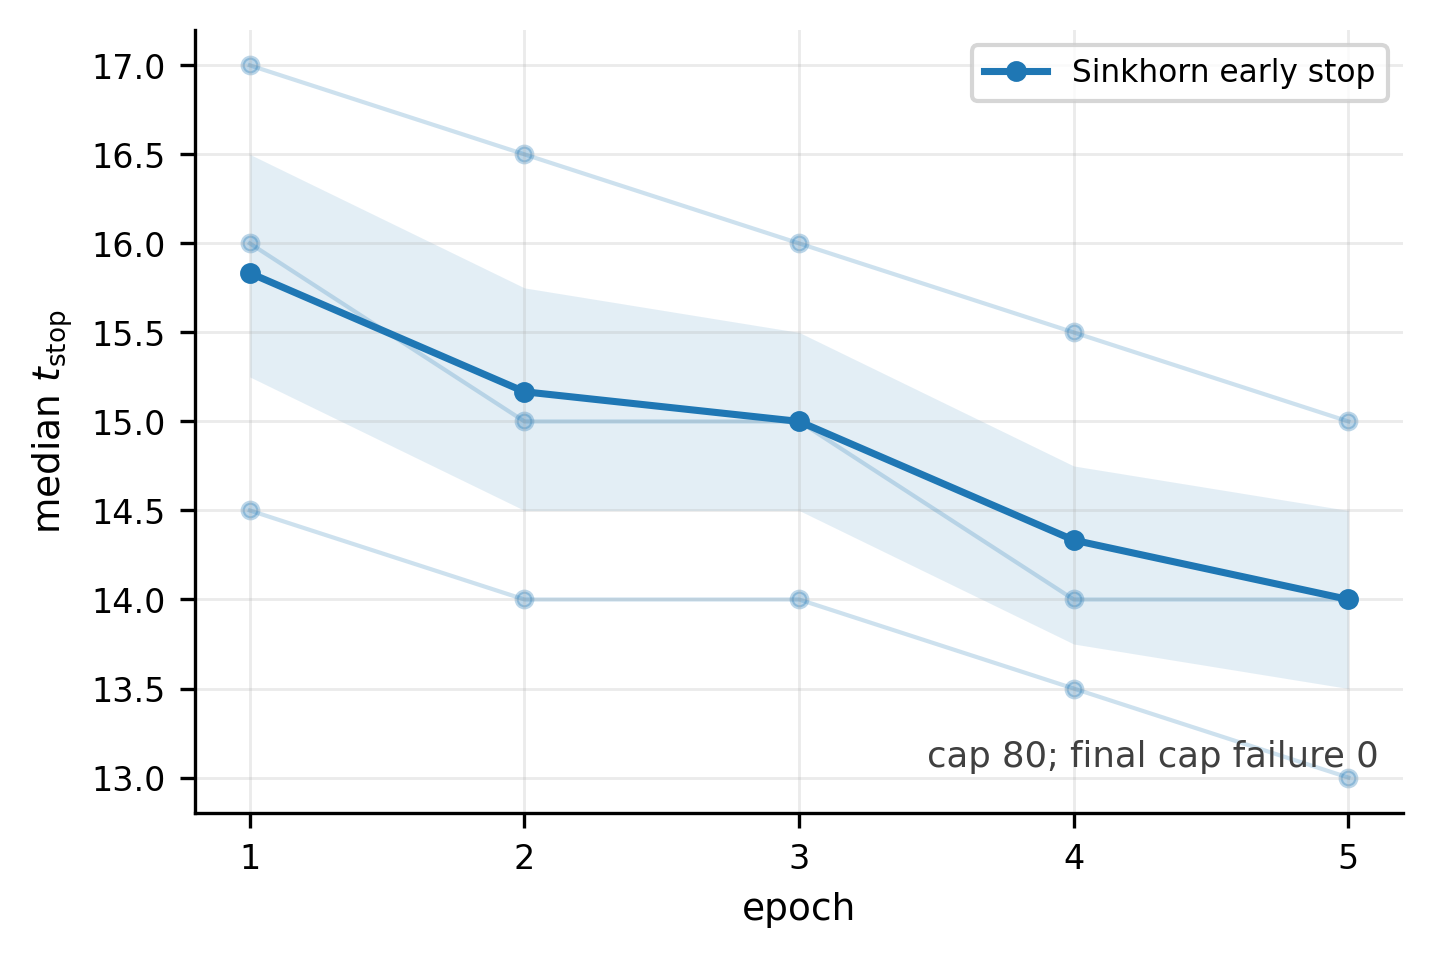
\includegraphics[width=\linewidth]{tstop_hist_early.png}
\small (d) Early-stop step counts.
\end{minipage}

\medskip
\captionof{figure}{Stress-run audit diagnostics for the finite-step Sinkhorn controller. These
plots use the same logs as the main certificate tables.}
\label{fig:stress-audit}
\end{center}
\FloatBarrier

\section{Auxiliary finite-step estimates}\label{app:auxiliary-estimates}

\paragraph{Proof of Lemma~\ref{lem:Psi}.}
Let \(a:=\max_i u_i\), \(b:=\min_i u_i\), and \(r:=a/b=e^\delta\ge1\).
The mean constraint gives \(b\le1\le a\). For the upper deviation, fixing the
ratio \(a/b=r\) and the mean, the largest possible value of \(a\) occurs when
one entry is \(a\) and the remaining \(n-1\) entries are \(b\). Thus
\[
        a\le \frac{nr}{r+n-1},
        \qquad
        a-1\le \frac{(n-1)(r-1)}{r+n-1}.
\]
For the lower deviation, the smallest possible value of \(b\) occurs when one
entry is \(b\) and the remaining \(n-1\) entries are \(a\). Thus
\[
        b\ge \frac{n}{1+(n-1)r},
        \qquad
        1-b\le \frac{(n-1)(r-1)}{1+(n-1)r}.
\]
Since \(1+(n-1)r\ge r+n-1\) for \(n\ge2\) and \(r\ge1\), the lower-tail bound is
no larger than the upper-tail bound. Therefore
\[
        \|u-\ones\|_{\infty,\mathrm{vec}}
        \le
        \frac{(n-1)(r-1)}{r+n-1}
        =\Psi_n(\delta).
\]
Solving \(\Psi_n(\delta)\le\varepsilon\) for \(r=e^\delta\) gives
\eqref{eq:Psi-inv}.

\paragraph{Proof of Lemma~\ref{lem:Gamma}.}
Since \(z=\Pi\log u\) and \(n^{-1}\sum_i u_i=1\), there is a unique scalar
normalization such that
\[
        u_i=\frac{n e^{z_i}}{\sum_{k=1}^n e^{z_k}}.
\]
We first maximize a single coordinate. Under the constraints \(\sum_i z_i=0\)
and \(\|z\|_2\le\eta\), the largest possible value of one coordinate is
\[
        a=\sqrt{\frac{n-1}{n}}\,\eta,
\]
attained when the remaining coordinates all equal \(-a/(n-1)\). Indeed, if
\(z_i=a\) is fixed, the sum of the other coordinates is \(-a\); Jensen's
inequality gives
\[
        \sum_{k\ne i}e^{z_k}
        \ge
        (n-1)e^{-a/(n-1)},
\]
with equality exactly in the equal-tail configuration. Therefore
\[
        u_i
        \le
        \frac{n e^a}{e^a+(n-1)e^{-a/(n-1)}}.
\]
This gives the upper-tail deviation \(\Gamma_n^+(\eta)\).

For the lower tail, two complementary estimates are useful. First, let
\(M=\max_i z_i\) and \(m=\min_i z_i\). For every coordinate,
\[
        u_i
        =
        \frac{n e^{z_i}}{\sum_k e^{z_k}}
        \ge
        \frac{n e^m}{n e^M}
        =
        e^{-(M-m)}.
\]
Since
\[
        M-m
        =
        \langle z,e_{i_{\max}}-e_{i_{\min}}\rangle
        \le
        \sqrt{2}\,\|z\|_2
        =
        \sqrt{2}\,\eta,
\]
we recover the global estimate
\[
        1-u_i\le1-e^{-\sqrt{2}\eta}.
\]

To obtain the correct first-order behavior, Cauchy--Schwarz and
\(\sum_i z_i=0\) give
\(|z_i|\le a=\sqrt{(n-1)/n}\,\eta\) for every coordinate. The elementary
Taylor remainder bound
\[
        e^x\le 1+x+\frac12 e^{|x|}x^2
\]
therefore gives
\[
        \frac1n\sum_{k=1}^n e^{z_k}
        \le
        1+\frac{e^a}{2n}\sum_{k=1}^n z_k^2
        =
        1+\frac{e^a}{2n}\eta^2.
\]
Together with \(z_i\ge-a\), this gives
\[
        u_i
        =
        \frac{e^{z_i}}{n^{-1}\sum_k e^{z_k}}
        \ge
        \frac{e^{-a}}{1+\frac{e^a}{2n}\eta^2}.
\]
Taking the better of the two valid lower bounds gives the stated
\(\Gamma_n^-(\eta)\). Since both \(\Gamma_n^+(\eta)\) and
\(\Gamma_n^-(\eta)\) have first-order coefficient
\(\sqrt{(n-1)/n}\), equation~\eqref{eq:Gamma-small} follows.

\subsection{Local finite-orbit derivative envelope}\label{app:local-envelope}

With the notation of Section~\ref{subsec:local-spectral}, consider the derivative on a neighborhood
of the Sinkhorn limit.

For \(x\in\ones^\perp\), define
\[
        g(x):=P^\top e^x,\qquad a(x):=P(g(x)^{-1}),
\]
and
\begin{equation}\label{eq:JF-JL}
        J_F(x):=
        \Pi\diag(a(x))^{-1}P\diag(g(x))^{-2}P^\top\diag(e^x)\Pi,
\end{equation}
\begin{equation}\label{eq:JL}
        J_L(x):=
        \Pi\diag(g(x))^{-1}P^\top\diag(e^x)\Pi .
\end{equation}
For \(R>0\), set
\begin{equation}\label{eq:rhoR-lambdaR}
        \rho_R:=\sup_{\substack{x\in\ones^\perp\\ \|x\|_2\le R}}\|J_F(x)\|_{2\to2},
        \qquad
        \lambda_R:=\sup_{\substack{x\in\ones^\perp\\ \|x\|_2\le R}}\|J_L(x)\|_{2\to2}.
\end{equation}

\begin{lemma}[Local spectral envelope]\label{lem:local-envelope}
Assume \(\rho_R<1\) and \(\|x_0\|_2\le R\). Then the Sinkhorn orbit remains in
\(\|x\|_2\le R\) and, for every \(t\ge1\),
\begin{equation}\label{eq:local-envelope-log}
        \|z_t\|_2\le\lambda_R\rho_R^{t-1}\|x_1-x_0\|_2 .
\end{equation}
Therefore,
\begin{equation}\label{eq:local-envelope-eps}
        \varepsilon_c^{(2t)}
        \le
        \Gamma_n\!\left(\lambda_R\rho_R^{t-1}\|x_1-x_0\|_2\right).
\end{equation}
The same bounds hold with certified upper bounds
\(\widehat\rho_R\ge\rho_R\), \(\widehat\lambda_R\ge\lambda_R\), provided
\(\widehat\rho_R<1\).
\end{lemma}

\begin{proof}
The displayed formulae for $J_F$ and $J_L$ are obtained by differentiating \eqref{eq:F-L-defs}. Because $\mathcal F(0)=0$, the mean-value theorem gives, for any $x\in\ones^\perp$ with $\|x\|_2\le R$,
\[
        \|\mathcal F(x)\|_2
        \le
        \rho_R\|x\|_2 .
\]
Thus the ball is invariant whenever $\rho_R<1$. Applying the same mean-value estimate to the differences gives
\[
        \|x_{s+1}-x_s\|_2
        \le
        \rho_R\|x_s-x_{s-1}\|_2,
        \qquad s\ge1,
\]
and therefore
\[
        \|x_t-x_{t-1}\|_2
        \le
        \rho_R^{t-1}\|x_1-x_0\|_2 .
\]
Since $z_t=\mathcal L(x_t)-\mathcal L(x_{t-1})$, another mean-value estimate gives \eqref{eq:local-envelope-log}. Lemma~\ref{lem:Gamma} converts the centered logarithmic error into the ordinary column-sum error.
\end{proof}

\paragraph{Orbit-wise derivative bound.}
Let $x_0,x_1,\dots,x_t$ be the actual logarithmic Sinkhorn orbit and define
\[
        \rho_s
        :=
        \sup_{0\le\theta\le1}
        \left\|
        J_F\big((1-\theta)x_{s-1}+\theta x_s\big)
        \right\|_{2\to2},
        \qquad s\ge1,
\]
\[
        \lambda_t^{\mathrm{seg}}
        :=
        \sup_{0\le\theta\le1}
        \left\|
        J_L\big((1-\theta)x_{t-1}+\theta x_t\big)
        \right\|_{2\to2}.
\]
Then
\begin{equation}\label{eq:orbitwise-log-cert}
        \|z_t\|_2
        \le
        \lambda_t^{\mathrm{seg}}
        \left(\prod_{s=1}^{t-1}\rho_s\right)
        \|x_1-x_0\|_2,
\end{equation}
and thus
\begin{equation}\label{eq:orbitwise-eps-cert}
        \varepsilon_c^{(2t)}
        \le
        \Gamma_n\!\left(
        \lambda_t^{\mathrm{seg}}
        \left(\prod_{s=1}^{t-1}\rho_s\right)
        \|x_1-x_0\|_2
        \right).
\end{equation}
This a posteriori bound replaces the global dynamic-range rate by derivative norms along the realized orbit.

Applying the mean-value theorem on each orbit segment and then Lemma~\ref{lem:Gamma} gives the stated bound.

\section{Predictor expansion and full-block bounds}\label{app:predictor-jacobian}

\subsection{Second-order local predictor formulas}\label{app:second-order-predictor}

The second-order diagnostic predictor keeps the quadratic terms in the
logarithmic Sinkhorn map.  With \(K=PP^\top\), define
\begin{equation}\label{eq:QF-QL}
        Q_F(x)
        :=
        -P\big((P^\top x)^{\odot2}\big)
        +\frac12 K(x^{\odot2})
        +\frac12 (Kx)^{\odot2},
\end{equation}
\begin{equation}\label{eq:QL}
        Q_L(x)
        :=
        \frac12 P^\top(x^{\odot2})
        -\frac12 (P^\top x)^{\odot2}.
\end{equation}
Then
\begin{equation}\label{eq:F-L-second-expansion}
        \mathcal F(x)=Kx+\Pi Q_F(x)+O(\|x\|^3),
        \qquad
        \mathcal L(x)=\Pi P^\top x+\Pi Q_L(x)+O(\|x\|^3).
\end{equation}
Set
\begin{equation}\label{eq:second-order-x}
        x_t^{[1]}:=K^t x_0,
        \qquad
        x_t^{[2]}
        :=
        K^t x_0+
        \sum_{s=0}^{t-1}K^{t-1-s}\Pi Q_F(K^s x_0).
\end{equation}
The second-order centered log-column predictor is
\begin{equation}\label{eq:second-order-predictor-log}
        \ell_t^{[2]}
        :=
        \Pi\Big[
        P^\top x_t^{[2]}+Q_L(x_t^{[1]})
        -P^\top x_{t-1}^{[2]}-Q_L(x_{t-1}^{[1]})
        \Big].
\end{equation}
We then define
\begin{equation}\label{eq:second-order-predictor-eps}
        \widehat v_t^{[2]}
        :=
        \frac{n\exp(\ell_t^{[2]})}{\sum_{j=1}^n\exp((\ell_t^{[2]})_j)},
        \qquad
        \widehat\varepsilon_{c,2}^{(2t)}
        :=
        \|\widehat v_t^{[2]}-\ones\|_{\infty,\mathrm{vec}}.
\end{equation}
For each fixed \(t\),
\begin{equation}\label{eq:second-order-accuracy}
        z_t=\ell_t^{[2]}+O_t(\|x_0\|^3).
\end{equation}
Thus \eqref{eq:second-order-predictor-eps} is the finite-step prediction
to compare with early numerical points, while
\eqref{eq:local-spectral-predicted-error} gives the asymptotic slope.


\subsection{Full-layer Jacobian \Amax bounds}\label{app:jacobian}

The mixer-product certificates in Section~\ref{sec:amax} isolate the contribution of stream mixing.
Full-network certificates additionally require independent control of the nonlinear
residual branch. We first record the generic composition bound, then give the
row-major Jacobian calculation for the mHC-style layer in \eqref{eq:mhc-layer}.

\begin{proposition}[Full-block \Amax composition bound]\label{prop:full-block-amax}
Consider a depth-$L$ network of the form
\begin{equation}\label{eq:full-block-generic}
        X_\ell=H^{(\ell)}X_{\ell-1}+\mathcal F_\ell(X_{\ell-1}),
        \qquad \ell=1,\dots,L,
\end{equation}
where $H^{(\ell)}\in\R^{n\times n}$ mixes streams and $\mathcal F_\ell$ denotes the remaining nonlinear part of the block. Suppose
\begin{equation}\label{eq:F-forward-lip}
        \Amax(\mathcal F_\ell(X)-\mathcal F_\ell(Y))
        \le a_\ell\Amax(X-Y)
\end{equation}
for all relevant $X,Y$. Then
\begin{equation}\label{eq:full-forward-bound}
        \Amax(X_L-Y_L)
        \le
        \prod_{\ell=1}^L\bigl(\|H^{(\ell)}\|_\infty+a_\ell\bigr)
        \Amax(X_0-Y_0).
\end{equation}
If, in addition, along the realized trajectory the adjoint Jacobian of the nonlinear branch satisfies
\begin{equation}\label{eq:F-backward-lip}
        \Amax\!\left(D\mathcal F_\ell(X_{\ell-1})^*G\right)
        \le b_\ell\Amax(G),
\end{equation}
then the input-gradient amplification obeys
\begin{equation}\label{eq:full-backward-bound}
        \Amax(\nabla_{X_0}\mathcal L)
        \le
        \prod_{\ell=1}^L\bigl(\|H^{(\ell)}\|_1+b_\ell\bigr)
        \Amax(\nabla_{X_L}\mathcal L).
\end{equation}
In particular, if $H^{(\ell)}\ge0$ is $(\varepsilon_r^{(\ell)},\varepsilon_c^{(\ell)})$-doubly stochastic, then
\begin{equation}\label{eq:full-block-marginal-bound}
        \Amax(\nabla_{X_0}\mathcal L)
        \le
        \prod_{\ell=1}^L\bigl(1+\varepsilon_c^{(\ell)}+b_\ell\bigr)
        \Amax(\nabla_{X_L}\mathcal L).
\end{equation}
\end{proposition}

\begin{proof}
Subtracting two trajectories and using the triangle inequality gives
\[
\begin{aligned}
\Amax(X_\ell-Y_\ell)
&\le \Amax\bigl(H^{(\ell)}(X_{\ell-1}-Y_{\ell-1})\bigr)
 +\Amax\bigl(\mathcal F_\ell(X_{\ell-1})-\mathcal F_\ell(Y_{\ell-1})\bigr)\\
&\le \bigl(\|H^{(\ell)}\|_\infty+a_\ell\bigr)\Amax(X_{\ell-1}-Y_{\ell-1}),
\end{aligned}
\]
which iterates to \eqref{eq:full-forward-bound}. The backward recursion has the form
\[
        G_{\ell-1}=(H^{(\ell)})^\top G_\ell+D\mathcal F_\ell(X_{\ell-1})^*G_\ell.
\]
Using \eqref{eq:amax-norm-link-backward} and \eqref{eq:F-backward-lip} gives
\[
        \Amax(G_{\ell-1})
        \le \bigl(\|H^{(\ell)}\|_1+b_\ell\bigr)\Amax(G_\ell),
\]
and iteration gives \eqref{eq:full-backward-bound}. The marginal version follows from \eqref{eq:amax_fact_inline}.
\end{proof}


Let $X\in\R^{n\times C}$ and define the row-major vectorization
\begin{equation}
\vecop_r(X):=\vecop(X^\top)\in\R^{nC},
\end{equation}
where $\vecop$ is the standard column-stacking operator.
With this convention one has, whenever products are well-defined,
\begin{equation}\label{eq:rvec-axb}
\vecop_r(AXB)=(A\otimes B^\top)\vecop_r(X),
\end{equation}
and in particular
\begin{equation}\label{eq:rvec-hx}
\vecop_r(HX)=(H\otimes I_C)\vecop_r(X).
\end{equation}


\paragraph{Layer Jacobian and induced-norm bounds}
Fix a layer $\ell$. Let $\Hres^{(\ell)}\in\R^{n\times n}$ be the residual mixer and
$\Hpre^{(\ell)},\Hpost^{(\ell)}\in\R^{1\times n}$ the pre/post aggregation row vectors.
Let $F^{(\ell)}:\R^{C}\to\R^{C}$ denote the feature map applied to the aggregated feature vector
$u:=\Hpre^{(\ell)}X\in\R^{C}$, and let $J_F^{(\ell)}\in\R^{C\times C}$ be the Jacobian of $F^{(\ell)}$ with respect to $u$.

The layer update is
\begin{equation}
X \mapsto \Hres^{(\ell)}X + \Hpost^{(\ell)\top}F^{(\ell)}(\Hpre^{(\ell)}X).
\end{equation}
Applying Equation~\eqref{eq:rvec-axb} and the chain rule gives the Jacobian (with respect to $\vecop_r(X)$):
\begin{align}\label{eq:jac}
J^{(\ell)}
&=
\Hres^{(\ell)}\otimes I_C
+
\big(\Hpost^{(\ell)\top}\otimes I_C\big)\,
J_F^{(\ell)}\,
\big(\Hpre^{(\ell)}\otimes I_C\big)\\
&=
\Hres^{(\ell)}\otimes I_C
+
\big(\Hpost^{(\ell)\top}\Hpre^{(\ell)}\big)\otimes J_F^{(\ell)},
\nonumber
\end{align}
where the second line uses $J_F^{(\ell)}=[1]\otimes J_F^{(\ell)}$ and the
mixed-product identity for Kronecker products.

\begin{proposition}[Layer Jacobian induced-norm bounds]\label{prop:full-jac}
With the notation above,
\begin{equation}\label{eq:jac-inf}
\norm{J^{(\ell)}}_{\infty}
\le
\norm{\Hres^{(\ell)}}_{\infty}
+
\norm{\Hpost^{(\ell)}}_{\infty,\mathrm{vec}}\,
\norm{J_F^{(\ell)}}_{\infty}\,
\norm{\Hpre^{(\ell)}}_{1,\mathrm{vec}}.
\end{equation}
Similarly,
\begin{equation}\label{eq:jac-one}
\norm{J^{(\ell)}}_{1}
\le
\norm{\Hres^{(\ell)}}_{1}
+
\norm{\Hpost^{(\ell)}}_{1,\mathrm{vec}}\,
\norm{J_F^{(\ell)}}_{1}\,
\norm{\Hpre^{(\ell)}}_{\infty,\mathrm{vec}}.
\end{equation}
\end{proposition}

\begin{proof}
The Kronecker factorization in \eqref{eq:jac} gives an exact norm identity for
the nonlinear rank-one stream term. Namely,
\[
\begin{aligned}
\left\|
\big(\Hpost^{(\ell)\top}\Hpre^{(\ell)}\big)\otimes J_F^{(\ell)}
\right\|_\infty
&=
\|\Hpost^{(\ell)\top}\Hpre^{(\ell)}\|_\infty
\|J_F^{(\ell)}\|_\infty\\
&=
\|\Hpost^{(\ell)}\|_{\infty,\mathrm{vec}}
\|\Hpre^{(\ell)}\|_{1,\mathrm{vec}}
\|J_F^{(\ell)}\|_\infty.
\end{aligned}
\]
Together with $\|\Hres^{(\ell)}\otimes I_C\|_\infty=\|\Hres^{(\ell)}\|_\infty$
and the triangle inequality, this proves \eqref{eq:jac-inf}. Similarly,
\[
\left\|
\big(\Hpost^{(\ell)\top}\Hpre^{(\ell)}\big)\otimes J_F^{(\ell)}
\right\|_1
=
\|\Hpost^{(\ell)}\|_{1,\mathrm{vec}}
\|\Hpre^{(\ell)}\|_{\infty,\mathrm{vec}}
\|J_F^{(\ell)}\|_1,
\]
which gives \eqref{eq:jac-one}. The only remaining slack in these layerwise
bounds is the triangle inequality between the residual and nonlinear Jacobian
terms.
\end{proof}

\begin{corollary}[Conditional full-block Jacobian certification]\label{cor:jacobian-cert}
Assume each residual mixer is entrywise nonnegative and $(\varepsilon_r^{(\ell)},\varepsilon_c^{(\ell)})$-doubly stochastic, so that
$\norm{\Hres^{(\ell)}}_\infty\le 1+\varepsilon_r^{(\ell)}$ and
$\norm{\Hres^{(\ell)}}_1\le 1+\varepsilon_c^{(\ell)}$. If, in addition, there exist constants
$b_{\mathrm{pre}},b_{\mathrm{post}},L_F\ge 0$ such that for all layers $\ell$,
\begin{equation}\label{eq:jac-assumptions}
\norm{\Hpre^{(\ell)}}_{1,\mathrm{vec}}\le b_{\mathrm{pre}},
\qquad
\norm{\Hpost^{(\ell)}}_{\infty,\mathrm{vec}}\le b_{\mathrm{post}},
\qquad
\norm{J_F^{(\ell)}}_\infty \le L_F,
\end{equation}
then
\begin{equation}\label{eq:jac-cert}
\norm{J^{(\ell)}}_\infty
\le
(1+\varepsilon_r^{(\ell)}) + b_{\mathrm{post}}\,L_F\,b_{\mathrm{pre}}.
\end{equation}
Thus
\begin{equation}
\norm{J^{(L)}\cdots J^{(1)}}_\infty
\le
\prod_{\ell=1}^L\Big((1+\varepsilon_r^{(\ell)}) + b_{\mathrm{post}}\,L_F\,b_{\mathrm{pre}}\Big).
\end{equation}
The backward induced-norm product has the parallel bound
\begin{equation}\label{eq:jac-cert-one-product}
\norm{J^{(L)}\cdots J^{(1)}}_1
\le
\prod_{\ell=1}^L
\left(
1+\varepsilon_c^{(\ell)}
+
\norm{\Hpost^{(\ell)}}_{1,\mathrm{vec}}
\norm{J_F^{(\ell)}}_1
\norm{\Hpre^{(\ell)}}_{\infty,\mathrm{vec}}
\right).
\end{equation}
\end{corollary}

Here $L_F$ is an architecture-dependent bound on the nonlinear block Jacobian.
For a pointwise MLP, it can be estimated from the induced norms of the affine maps
and the Lipschitz constants of the activations. For an attention block, it also depends
on the projection operators and the data-dependent attention map. The full-block
certificate therefore retains $L_F$ explicitly rather than assigning it a universal value.




\end{document}
